\documentclass[twoside]{article}


\usepackage[T2A]{fontenc}                   %!? закрепляет внутреннюю кодировку LaTeX
\usepackage[utf8]{inputenc}                 %!  закрепляет кодировку utf8
\usepackage[russian,english]{babel}         %!  подключает русский и английский
\usepackage[margin=1.8cm]{geometry}         %!  фиксирует оступ на 2cm

\usepackage[unicode, pdftex]{hyperref}      %!  оглавление для панели навигации по PDF-документу + гиперссылки

\usepackage{amsthm}                         %!  newtheorem и их сквозная нумерация
\usepackage{hypcap}                         %?  адресация на картинку, а не на подпись к ней
\usepackage{caption}                        %-  позволяет корректировать caption 
\usepackage{fancyhdr}                       %   добавить верхний и нижний колонтитул
\usepackage{wrapfig}                        %!  обтекание таблиц и рисунков

\usepackage{amsmath}                        %!  |
\usepackage{amssymb,textcomp, esvect,esint} %!  |важно для формул 
\usepackage{amsfonts}                       %!  математические шрифты
\usepackage{mathrsfs}                       %  добавит красивые E, H, L
% \usepackage{ulem}                           %!  перечеркивание текста
\usepackage{abraces}                        %?  фигурные скобки сверху или снизу текста
\usepackage{pifont}                         %!  нужен для крестика
\usepackage{cancel}                         %!  аутентичное перечеркивание текста
\usepackage{esvect}                         %  добавит вектора стрелочками

\usepackage{graphicx}                       %?  графическое изменение текста
\usepackage{indentfirst}                    %   добавить indent перед первым параграфом
\usepackage{xcolor}                         %   добавляет цвета
\usepackage{enumitem}                       %!  задание макета перечня.

\usepackage{booktabs}                       %!  добавляет книжные линии в таблицы
% \usepackage{multirow}                       %   объединение ячеек в таблицах
% \usepackage{tikz}                           %!  высокоуровневые рисунки (кружочек)
% \usepackage{import}                         %   |
% \usepackage{xifthen}                        %   |
% \usepackage{pdfpages}                       %   | вставка рисунков pdf_tex
% \usepackage{transparent}                    %   |

\usepackage{bbm}                            %   добавляет \mathbbm{1}

% \newtheorem{to_thr}{Thr}[section]
% \newtheorem{to_suj}[to_thr]{Suj}
% \newtheorem{to_lem}[to_thr]{Lem}
% \newtheorem{to_com}[to_thr]{Com}
% \newtheorem{to_con}[to_thr]{Con}
% \theoremstyle{definition}
% \newtheorem{to_def}[to_thr]{Def}


\newenvironment{itemize*}
{
    \vspace{-\topsep}
    \begin{itemize}
        \setlength{\itemsep}{1pt}
        \setlength{\parskip}{1pt}
        }
    {\end{itemize}
}

\newenvironment{enumerate*}
{
    \vspace{-\topsep}
    \begin{enumerate}
        \setlength{\itemsep}{1pt}
        \setlength{\parskip}{1pt}}
    {\end{enumerate}
}

% \newenvironment{description*}
% {
%     \begin{description}
%         \setlength{\itemsep}{1pt}
%         \setlength{\parskip}{1pt}}
%     {\end{description}
% }

\definecolor{ugrey}{HTML}{666666}
% \definecolor{ublue}{HTML}{08088A}
% \definecolor{linkcolor}{HTML}{0000CC}
% \definecolor{urlcolor}{HTML}{006600}
% \hypersetup{
%     pdfstartview=FitH,  
%     linkcolor=linkcolor,
%     urlcolor=urlcolor, 
%     colorlinks=true,
%     citecolor=blue}
% базовая подстройка
\renewcommand{\d}{\, d}
\renewcommand{\leq}{\leqslant}
\renewcommand{\geq}{\geqslant}


% авторские команды
\newcommand{\vc}[1]{\boldsymbol{#1}}
\newcommand{\1}{\mathbbm{1}}
\newcommand{\T}{^{\textnormal{T}}}
\newcommand{\D}{^{\dag}}
\newcommand{\sub}[2]{#1_{\textnormal{#2}}}
\newcommand{\vp}{\vphantom{\dfrac{1}{2}}}
\newcommand{\hc}{\mathrm{h.c.}}

% операторы (просто прямой текст)
\renewcommand{\Im}{\mathop{\mathrm{Im}}\nolimits}
\renewcommand{\Re}{\mathop{\mathrm{Re}}\nolimits}
% \renewcommand{\P}{\mathop{\mathrm{P}}\nolimits}
% \newcommand{\E}{\mathop{\mathrm{E}}\nolimits}
% \newcommand{\D}{\mathop{\mathrm{D}}\nolimits}
% \newcommand{\cov}{\mathop{\mathrm{cov}}\nolimits}
\newcommand{\diag}{\mathop{\mathrm{diag}}\nolimits}
\newcommand{\std}{\mathop{\mathrm{std}}\nolimits}
\newcommand{\mean}{\mathop{\mathrm{mean}}\nolimits}
\newcommand{\sigmoid}{\mathop{\mathrm{sigmoid}}\nolimits}
\newcommand{\card}{\mathop{\mathrm{card}}\nolimits}
\newcommand{\grad}{\mathop{\mathrm{grad}}\nolimits}
\renewcommand{\div}{\mathop{\mathrm{div}}\nolimits}
\newcommand{\rot}{\mathop{\mathrm{rot}}\nolimits}
\newcommand{\Ker}{\mathop{\mathrm{ker}}\nolimits}
\newcommand{\spec}{\mathop{\mathrm{spec}}\nolimits}
\newcommand{\sign}{\mathop{\mathrm{sign}}\nolimits}
\newcommand{\tr}{\mathop{\mathrm{tr}}\nolimits}
\newcommand{\rg}{\mathop{\mathrm{rg}}\nolimits}
\newcommand{\const}{\textnormal{const}}


% цветной текст
\newcommand{\grey}[1]{\textcolor{ugrey}{#1}}
\newcommand{\red}[1]{\textcolor{red}{#1}}
\newcommand{\green}[1]{\textcolor{urlcolor}{#1}}
\newcommand{\blue}[1]{\textcolor{ublue}{#1}}


% символы
\newcommand{\cmark}{\text{\ding{51}}}
\newcommand{\xmark}{\text{\ding{55}}}


% подгрузка pdf_tex картинок
% \newcommand{\incfig}[1]{%
%     \def\svgwidth{\columnwidth}
%     \import{./figures/}{#1.pdf_tex}
% }

\newcommand{\addletter}[2]{\begin{picture}(7,7) \put(0,#1){{#2)}} \end{picture}}



% специфично к квантам
\newcommand{\ket}[1]{\left| #1 \right\rangle}
\newcommand{\bra}[1]{\left\langle #1 \right|}

% \newcommand{\dppp}{\frac{d^3 p}{(2 \pi \hbar)^3}}

\DeclareDocumentCommand{\bk}{m o m}{
    \IfNoValueTF{#2}{\langle #1 | #3 \rangle}{\langle #1 | #2 | #3 \rangle}
}
\newcommand{\kb}[2]{| #1 \rangle \langle #2 |}

\newcommand{\tth}{\sub{t}{th}}
% !TEX root = ../master-thesis.tex

% add page header

\pagestyle{fancy}
\fancyhf{}
% \fancyhead[RE,LO]{\thepage}
% \fancyhead[LE,RO]{Ж\raisebox{-1.5pt}{и}К}
% \fancyhead[CO,CE]{\nouppercase{\textit{\leftmark}}}
\fancyhead[LE,RO]{\nouppercase{\textit{\leftmark}}}
\fancyfoot[LE,RO]{\thepage}




\DeclareRobustCommand{\tmpsim}{ %%%%%%%%%%%%%% ~ < %%%%%%%%%%%%%%%%%%%
  \mathbin{\text{
      \raisebox{-1pt}{
            \hspace{-4.5pt} \rotatebox{-26}{\scalebox{0.8}[0.7]{$\sim$}}
        }
  }}
}
\def\lesim{{
    \setbox0\hbox{$\ <\ $}
    \rlap{\hbox to \wd0{\hss$\tmpsim$\hss}}\box0
}}
%%%%%%%%%%%%%%%%%%%%%%%%%%%%%%%%%%%%%%%%%%%%%%%%%%%%%%%%%%%%%%%%%%%%%%


\def\letuscom{%%%%%%%%%%%%%%%%%%%%%% ПУСТЬ %%%%%%%%%%%%%%%%%%%%%%%%%%
\mathord{\setbox0=\hbox{$\exists$}%
     \hbox{\kern 0.125\wd0%
           \vbox to \ht0{%
              \hrule width 0.75\wd0%
              \vfill%
              \hrule width 0.75\wd0}%
           \vrule height \ht0%
           \kern 0.125\wd0}%
   }%
}
\newcommand{\letus}{\raisebox{-1.2pt}{$\letuscom$}}
%%%%%%%%%%%%%%%%%%%%%%%%%%%%%%%%%%%%%%%%%%%%%%%%%%%%%%%%%%%%%%%%%%%%%%


\usepackage{arydshln} %%%%%%%%%%%%%%% ЛИНИИ В МАТРИЧКЕ %%%%%%%%%%%%%%%
\makeatletter
  \renewcommand*\env@matrix[1][*\c@MaxMatrixCols c]{%
    \hskip -\arraycolsep
    \let\@ifnextchar\new@ifnextchar
  \array{#1}}
\makeatother
%%%%%%%%%%%%%%%%%%%%%%%%%%%%%%%%%%%%%%%%%%%%%%%%%%%%%%%%%%%%%%%%%%%%%%


\makeatletter %%%%%%%%%%%%%%% КРУЖОЧЕК %%%%%%%%%%%%%%%%%%%%%%%%%%%%%%%
\newcommand*{\encircled}[1]{\relax\ifmmode\mathpalette
\@encircled@math{#1}\else\@encircled{#1}\fi}
\newcommand*{\@encircled@math}[2]{\@encircled{$\m@th#1#2$}}
\newcommand*{\@encircled}[1]{%
  \tikz[baseline,anchor=base]{\node[draw,circle,outer sep=0pt,
                                        inner sep=.2ex] {#1};}}
\makeatother
%%%%%%%%%%%%%%%%%%%%%%%%%%%%%%%%%%%%%%%%%%%%%%%%%%%%%%%%%%%%%%%%%%%%%%




\begin{document}

% set skip of equation length 

\setlength{\abovedisplayskip}{3pt}
\setlength{\abovedisplayshortskip}{3pt}
\setlength{\belowdisplayskip}{3pt}
\setlength{\belowdisplayshortskip}{3pt}
\setlength{\headheight}{13pt}

% \numberwithin{equation}{section}

% \renewcommand{\thesubsection}{\thesection.\alph{subsection}}

% document's head

\begin{center}
    \LARGE \textsc{Fermionic State Preparation and Imaging \\ in Optical Tweezer Array}
\end{center}

\hrule

\phantom{42}

\begin{flushright}
    \begin{tabular}{rr}
        % \textbf{Author}: 
        & Khoruzhii Kirill \\
        % & \\
    % date:
        % \textbf{Date}:
        & \textit{Munich, \today}\\
    \end{tabular}
\end{flushright}

\noindent
Quantum simulation with ultracold atoms requires both high-fidelity preparation of the initial many-body state and site-resolved measurement of the final state. This thesis presents the development of experimental techniques for spin-resolved free-space imaging and deterministic, spin-selective preparation of ultracold fermionic $^6$Li atoms in a two-dimensional optical tweezer array. The array is generated using crossed acousto-optic deflectors, with precise control achieved through a combination of direct camera-based calibration and atom-based feedback. A novel spilling method enables the preparation of arbitrary spin- and site-resolved occupation patterns. The thesis also introduces numerical tools for simulating Fermi-Hubbard dynamics in small systems, laying the groundwork for future out-of-equilibrium quantum simulation experiments.







\thispagestyle{empty}

\tableofcontents

% \vfill

% Базовая структура диплома:
% \begin{enumerate*}
%     \item deterministic state preparation (single tweezer)
%     \begin{enumerate*}
%         \item loading (2D MOT, MOT, Dipol Trap, Tweezer)
%         \item spilling
%     \end{enumerate*}
%     \item single-atom spin resolved free space imaging
%     \begin{enumerate*}
%         \item ! flashing and model
%         \item ! image processing
%     \end{enumerate*}
%     \item deterministic state preparation (tweezer array)
%     \begin{enumerate*}
%         \item ! generating
%         \item ! control
%         \item ! balancing
%     \end{enumerate*}
% \end{enumerate*}

% Это история про то как сделать и сфотографировать спиновое состояние в твизере.   

% Нужно выписать contributions! И им следовать.   




\newpage



% !TEX root = ../master-thesis.tex


\section*{Мысли про текст}

\begin{enumerate}
	\item Storyline
	\item Каждая картинка должна быть описана и понятна. 
	\item Описание unirand эксперимента: подробнее про структуру уровней, про картинки.
	% \item Вводный рассказ про Fermi Hubbard
	% \item Tweezer loading
	% \item Tweezer movement
	\item ? добавить в chapter 6 про добавки с finite size к термализации из эргодического бассейна
	% \item ? MWM
	% \item BMF as SAT task
	\item ? Написать про добавки к obj function в линейной модели
	
	% \item Atom based measurements: SVF, , atom-based crosstalk (and comparison)
	
	% \item site- and spin- resolved state preparation

	% \item non-factorizable state preparation, add large Li imgs (see movie)
	 % Можно а-ля the Li добавлять сверху к средним картинкам расшифровку

	% \item Графики для антенн с фитом

\end{enumerate}



\section*{Мысли про figures}


\begin{itemize}
	\item Setup description
	\item ! That needs to be justified, there could be couplings between H and V (via the angle of the beams entering the second AOD)
	\item ! Схема стабилизации лазеров, какие отстройки, какие частоты, в контексте imaging
	% \item Single atom counting
	\item Демонстрация с Random Unitaries (Xinyi тезис)
	\item Схема установки, фото 3D mot
	% \item BEC
	\item Imaging: разница двух облачков (один, два continous, два alternating)
	% \item Imaging: histogram noise vs atoms, raw nuvu img
	% \item Flashing. Экспериментальная установка, табличка с её параметрами
	% \item State preparation: spilling. Схематичное изображение (посмотреть в Heidelberg thesis).
	% \item ? Экспериментальная последовательность
	\item ? Feshbach resonance
	% \item ? loading issues
	\item ? MWM (simulation, observed)
	\item ? Theory: описание fermi-hubbard, фазовая диаграмма (посмотреть coepsill)
	\item ? Theory: вклад от лабиринтов в локализацию
	% \item ? 2D Step Plot
\end{itemize}



% Huang: 17-25
% Culemann: 15-24




% Sec.\ref{sec:intro} or subsection\ref{subsec:control} Fig.\ref{fig:stepplot} or \eqref{eq:evolution} \newpage


% % !TEX root = ../master-thesis.tex











% \newpage

% \begin{figure}[h]
%     \centering
%     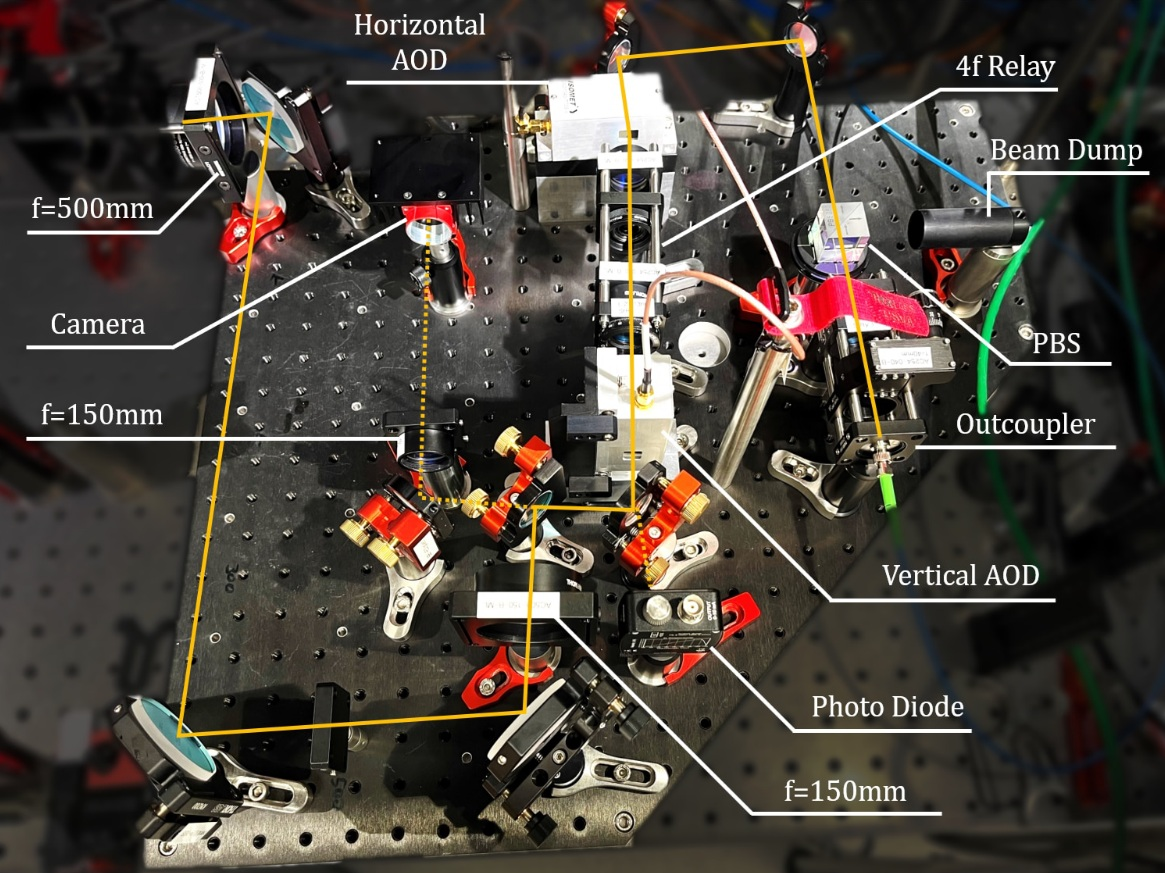
\includegraphics[width=0.5\textwidth]{imgs/tw-setup.jpg}
%     \caption{
%     \textbf{Optical setup for 2D tweezer array.} 
%     The beam path (solid orange line) includes two orthogonal AODs, a $4f$ relay, and diagnostic components. Dashed lines indicate monitoring light paths. Taken from \cite{culemann_construction_2024}.
%     }
%     \label{fig:tw-setup}
% \end{figure}


 












% \begin{figure}
%     \centering
%     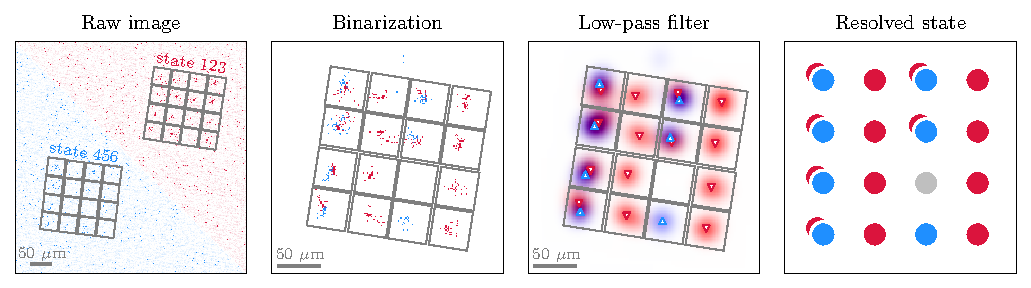
\includegraphics{fig-py/imaging-spin-resolved.pdf}
%     \caption{
%         \textbf{Spin-resolved single-atom imaging.}
%         Spatially separated $\sigma_+$ and $\sigma_-$ fluorescence is imaged onto two distinct regions of the camera. The binarization step identifies photon counts above a threshold, followed by a low-pass filter to extract spatially localized signals. Final spin states are assigned based on relative signal strength in each channel:
%         \raisebox{-1pt}{\scalebox{1.5}{\textcolor{ublue}{\textbullet}}} -- $\ket{1}$, 
%         \raisebox{-1pt}{\scalebox{1.5}{\textcolor{ured}{\textbullet}}} -- $\ket{2}$, 
%         \raisebox{-1pt}{\scalebox{1.5}{\textcolor{uhole}{\textbullet}}} -- no atom.
%     }
%     \label{fig:spin-resolved}
% \end{figure}


% Lorem ipsum dolor sit amet, consectetur adipisicing elit, sed do eiusmod
% tempor incididunt ut labore et dolore magna aliqua. Ut enim ad minim veniam,
% quis nostrud exercitation ullamco laboris nisi ut aliquip ex ea commodo
% consequat. Duis aute irure dolor in reprehenderit in voluptate velit esse
% cillum dolore eu fugiat nulla pariatur. Excepteur sint occaecat cupidatat non
% proident, sunt in culpa qui officia deserunt mollit anim id est laborum.


% \newline
% \phantom{42}
% \newline
% \addletter{100}{c} \phantom{4}
% 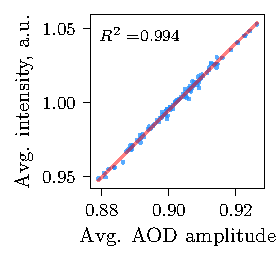
\includegraphics{fig-py/crosstalk-camera-amp.pdf}
% \phantom{4}
% \addletter{100}{d} \phantom{4}
% 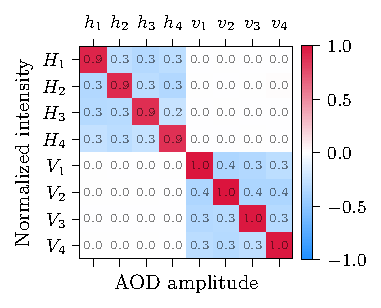
\includegraphics{fig-py/crosstalk-camera.pdf}
% \hfill
% \phantom{4}

 \newpage


\newpage
% --------------------------------------------------------------------------------------
\section{Introduction} \label{sec:intro}
% --------------------------------------------------------------------------------------
\subsection{The Fermi-Hubbard model}
% !TEX root = ../master-thesis.tex

% \textbf{High-temperature superconductivity.} 
The discovery of unconventional superconductivity in copper-oxide ceramics with critical temperatures reaching 135 K represents one of the most significant puzzles in condensed matter physics. These materials exhibit a complex phase diagram featuring strange metallic behavior that violates conventional Fermi liquid theory, pseudogap phenomena emerging from antiferromagnetic Mott insulating parent compounds, and the eventual emergence of d-wave superconductivity upon doping \cite{koepsell_quantum_2021}. Theoretical progress has been hampered by the strongly correlated nature of electrons in these systems, where simple perturbative approaches fail and the interplay between magnetic interactions, charge dynamics, and pairing mechanisms remains poorly understood.

The Fermi-Hubbard model, defined by the Hamiltonian
\begin{equation}
H = -t \sum_{\langle i,j \rangle, \sigma} \left( c_{i,\sigma}^\dagger c_{j,\sigma} + \text{h.c.} \right) + U \sum_i n_{i,\uparrow} n_{i,\downarrow} + \sum_{i,\sigma} \varepsilon_i n_{i,\sigma},
\end{equation}
captures the essential physics believed to underlie high-temperature superconductivity. The competition between kinetic energy (hopping amplitude $t$) and on-site Coulomb repulsion ($U$) gives rise to the rich phase diagram observed in cuprates, while site-dependent potentials $\varepsilon_i$ allow controlled introduction of disorder.

% \textbf{Quantum thermalization and localization.} 
Beyond equilibrium phenomena, the Fermi-Hubbard model serves as a paradigmatic system for understanding fundamental questions about quantum statistical mechanics in isolated many-body systems. The Eigenstate Thermalization Hypothesis (ETH) predicts that generic quantum systems evolve toward thermal equilibrium, with local observables losing memory of initial conditions \cite{deutsch_quantum_1991,srednicki_chaos_1994}. However, the presence of disorder can dramatically alter this behavior, leading to Anderson localization in non-interacting systems where all single-particle states become exponentially localized \cite{anderson_absence_1958,billy_direct_2008,roati_anderson_2008}. The interplay between interactions and disorder gives rise to many-body localization (MBL), a non-thermal phase where strongly interacting systems fail to thermalize despite high energy density \cite{basko_metalinsulator_2006,nandkishore_many-body_2015,abanin_colloquium_2019}. MBL systems exhibit characteristic logarithmic growth of entanglement entropy, violation of ETH, and persistent memory of initial conditions. Recent experimental observations of MBL signatures in both one- and two-dimensional ultracold atom systems have opened new avenues for studying these exotic quantum phases \cite{schreiber_observation_2015,choi_exploring_2016,bordia_probing_2017}.

% \textbf{Competition of energy scales.} 
% The rich physics of the Fermi-Hubbard model emerges from the competition between three characteristic energy scales: the kinetic energy set by the hopping amplitude $t$, the interaction energy characterized by the on-site repulsion $U$, and the disorder strength parameterized by the variance of $\varepsilon_i$. 
In the strongly interacting regime $U \gg t$, the system exhibits Mott insulating behavior with suppressed charge fluctuations and emergent magnetic ordering \cite{mazurenko_cold-atom_2017}. Weak disorder can enhance localization effects, while strong disorder can drive transitions between thermal and many-body localized phases. Understanding the dynamical phase diagram in the space of these competing energy scales represents one of a central challenges in quantum many-body physics.

\subsection{Experimental and computational challenges}
% !TEX root = ../master-thesis.tex

\textbf{Solid-state limitations.} Despite decades of intensive research, fundamental questions about high-temperature superconductivity and many-body localization remain unresolved due to inherent limitations of solid-state systems. Real materials possess complex crystal structures with multiple orbital degrees of freedom, phonon interactions, and intrinsic disorder that obscure the underlying electronic physics \cite{koepsell_quantum_2021}. The limited tunability of material parameters requires synthesizing new compounds for each point in parameter space, making systematic studies of phase diagrams challenging. Furthermore, many key observables remain experimentally inaccessible in solid-state systems. Higher-order spin correlations, real-space magnetic textures, and single-site resolved quantities cannot be directly measured using conventional condensed matter probes, which typically access momentum-space or bulk averaged properties.

\textbf{Computational intractability.} Classical numerical approaches face fundamental obstacles when simulating strongly correlated fermionic systems. The dimension of the Hilbert space grows exponentially with system size, rendering exact diagonalization feasible only for very small clusters. Quantum Monte Carlo methods, while successful for certain bosonic systems, suffer from the fermion sign problem in the presence of frustration or doping, leading to exponentially growing statistical errors \cite{koepsell_quantum_2021}. Approximate methods such as density matrix renormalization group (DMRG) work well in one dimension but become inefficient for two-dimensional systems due to area-law violations in entanglement entropy. These computational limitations severely constrain theoretical understanding of the parameter regimes most relevant to high-temperature superconductivity and many-body localization.

\textbf{Key observables needed.} Progress in understanding both equilibrium and dynamical properties of the Fermi-Hubbard model requires access to observables that are difficult or impossible to measure in conventional systems. For high-temperature superconductivity, key quantities include real-space spin-charge correlations that reveal magnetic polaron formation, site-resolved doping profiles, and the evolution of magnetic correlations with charge carrier density \cite{koepsell_quantum_2021}. For dynamical phase studies, essential observables include local particle densities $\langle n_i(t) \rangle$, magnetization profiles $\langle \sigma^z_i(t) \rangle$, and multi-point correlations that distinguish thermal, Anderson localized, and many-body localized phases. Additionally, investigating dynamical phases requires the ability to prepare arbitrary initial states, control disorder realizations, and perform extensive statistical averaging over many experimental repetitions to extract meaningful signals from noisy quantum dynamics.

\subsection{Ultracold atoms and the tweezer-based approach}
% !TEX root = ../master-thesis.tex

\textbf{Cold atoms advantages.} Ultracold atomic gases provide an exceptionally clean and tunable platform for realizing the Fermi-Hubbard model with unprecedented control over system parameters \cite{esslinger_fermi-hubbard_2010,gross_quantum_2017}. Neutral fermionic atoms such as $^6$Li trapped in optical lattices created by interfering laser beams naturally implement the kinetic energy term through tunneling between neighboring sites. The interaction strength $U$ can be continuously tuned using Feshbach resonances, where an external magnetic field controls the scattering length between atoms in different hyperfine spin states. This allows experimental exploration of the entire phase diagram from the non-interacting limit to strongly correlated regimes. Site-dependent potentials can be introduced using digital micromirror devices or spatial light modulators, enabling controlled studies of disorder effects and many-body localization \cite{choi_exploring_2016,schreiber_observation_2015}.

The development of quantum gas microscopy has revolutionized the field by providing single-site resolution imaging of atomic lattice systems \cite{bakr_quantum_2009,sherson_single-atom-resolved_2010}. These techniques enable direct measurement of local observables such as density correlations, magnetic structure factors, and spin-resolved occupations that are inaccessible in solid-state systems \cite{gross_quantum_2021}. Recent achievements include the observation of antiferromagnetic correlations in two-dimensional Fermi-Hubbard systems \cite{mazurenko_cold-atom_2017,parsons_site-resolved_2016} and demonstrations of many-body localization in disordered lattices \cite{bordia_probing_2017}.

\textbf{Current limitations.} Despite these advances, conventional optical lattice experiments face fundamental constraints in state preparation that limit their potential for studying complex many-body phenomena. Thermal loading from magneto-optical traps produces statistical filling with Poissonian atom number fluctuations, resulting in random defects and uncontrolled entropy that obscure the underlying physics \cite{esslinger_fermi-hubbard_2010}. The harmonic confinement typically present in these systems creates spatial inhomogeneity through varying local chemical potential, leading to "wedding cake" structures with different filling factors across the trap. Additionally, achieving specific initial states required for studying dynamical phases or controlled doping profiles remains challenging with conventional loading methods.

\textbf{Tweezer innovation.} Optical tweezer arrays offer a transformative solution to these state preparation challenges by enabling deterministic, bottom-up assembly of many-body quantum systems \cite{browaeys_many-body_2020}. Individual atoms can be captured and manipulated in tightly focused laser beams, providing single-site control over both spatial and internal degrees of freedom. Recent demonstrations have shown the feasibility of implementing few-body Fermi-Hubbard dynamics in programmable tweezer geometries \cite{spar_realization_2022,yan_two-dimensional_2022}, establishing the foundation for scalable fermionic quantum simulators.

This work advances tweezer-based approaches through the development of crossed acousto-optic deflector (AOD) systems that enable rapid reconfiguration of two-dimensional arrays. The key innovation lies in implementing spin-selective manipulation protocols that allow preparation of arbitrary site- and spin-resolved occupation patterns. Combined with novel imaging techniques for spin-resolved single-shot detection, this platform provides the experimental tools necessary for systematic studies of both equilibrium and dynamical Fermi-Hubbard physics.

\textbf{Separation of preparation and dynamics.} The tweezer-based approach exploits a fundamental insight: optimal state preparation and Hamiltonian evolution can be achieved using different experimental configurations. High-fidelity initial state preparation is performed in the tweezer array, where strong confinement and individual site control enable deterministic loading and spin manipulation. Subsequently, atoms are transferred to an optical lattice optimized for implementing the desired Hamiltonian evolution with precise control over tunneling and interaction parameters. This separation enables access to low-entropy initial states that would be statistically unlikely under thermal loading, opening new possibilities for studying quantum phase transitions, out-of-equilibrium dynamics, and exotic correlated phases.

\subsection{Thesis contributions and outlook}
% !TEX root = ../master-thesis.tex

% \textbf{Technical innovations developed.} 
This work addresses the key experimental bottlenecks limiting progress in Fermi-Hubbard quantum simulation through the development of three interconnected technological advances. The first innovation is a spin-resolved free-space imaging system for $^6$Li atoms that enables simultaneous detection of both hyperfine ground states in a single experimental shot. Unlike previous sequential imaging approaches \cite{bergschneider_spin-resolved_2018}, the implementation utilizes stretched states $|3\rangle$ and $|6\rangle$ with polarization-selective detection paths, achieving \red{99\%} spin discrimination fidelity while maintaining fast imaging times of 20 $\mu$s. This capability provides direct access to local magnetization and spin correlations essential for characterizing magnetic phases and dynamical regimes.

The second major contribution involves the design and control of two-dimensional optical tweezer arrays using crossed acousto-optic deflectors. This work develops calibration protocols that achieve uniform tweezer depths across arrays. A key innovation is the implementation of spin-selective spilling techniques that exploit differential magnetic moments of hyperfine states to enable deterministic preparation of arbitrary site- and spin-resolved occupation patterns. This approach represents the first demonstration of programmable spin-selective state preparation using crossed AOD configurations.

The third component consists of numerical simulation tools that provide theoretical benchmarks for experimental protocols. A custom GPU-accelerated software package was developed that combines exact diagonalization with Krylov subspace methods, enabling simulation of Fermi-Hubbard dynamics in systems up to $10^9$ dimensions. The package supports arbitrary geometries while efficiently computing observables including local densities, spin correlations, and entanglement entropy.

% \textbf{Numerical roadmap for dynamical phases.} 
The computational framework developed in this work serves as both a validation tool for experimental protocols and a roadmap for near-term studies of quantum thermalization and localization. Systematic simulations demonstrate clear signatures that distinguish thermal, Anderson localized, and many-body localized phases through experimentally accessible observables such as imbalance relaxation and entanglement growth. These results provide concrete targets for upcoming experiments and establish the parameter regimes where different dynamical behaviors can be reliably observed with the developed experimental tools.

% \textbf{Thesis statement.} 
This work develops key experimental tools for studying both equilibrium and dynamical aspects of the Fermi-Hubbard model in ultracold atomic systems. By combining deterministic state preparation in programmable tweezer arrays with spin-resolved imaging, the platform enables systematic investigation of magnetic correlations relevant to quantum thermalization phenomena in strongly correlated fermions.

% \textbf{Chapter roadmap.} 
The experimental platform and its capabilities are presented through a sequence of technical developments that build toward the physics applications. Section 2 provides an overview of the overall experimental apparatus. Section 3 details the implementation of spin-resolved free-space imaging, including the optical setup, image processing algorithms, and characterization of detection fidelity. Section 4 describes the tweezer array system, covering AOD control, calibration procedures, and spin-selective state preparation protocols. Section 5 presents the numerical simulation framework and demonstrates its application to studies of dynamical phases in small Fermi-Hubbard systems. Together, these tools establish a foundation for future studies of strongly correlated quantum matter using fermionic systems.

% 
\subsection{Thesis outline}

This thesis describes the development of experimental and computational tools for the preparation and probing of fermionic many-body states in a programmable optical tweezer array. The overarching goal is to enable bottom-up quantum simulation of lattice models, with precise control over initial conditions and single-atom, spin-resolved readout.

Sec.~\ref{sec:imaging} presents the implementation of spin-resolved single-atom imaging of $^6$Li in free space. The section describes the optical layout, the image processing pipeline, and introduces the Su-Schrieffer-Heeger model as a conceptual framework for understanding spin-dependent imaging dynamics.

Sec.~\ref{sec:tweezer} focuses on the creation and control of two-dimensional tweezer arrays. The section begins with the optical setup and AOD control, followed by a detailed discussion of calibration procedures and tweezer depth balancing using both camera-based and atom-based feedback. A key result is the development of a spin-selective spilling technique, enabling the preparation of spin- and site-resolved occupation patterns. Arbitrary configurations are realized through iterative removal steps, formalized via boolean matrix factorization.

Sec.~\ref{sec:mwm} introduces the concept of a matter-wave magnifier—a lensing scheme designed to enhance spatial resolution for future lattice imaging. Although not yet implemented experimentally, fast simulations of wavefunction propagation and Monte Carlo sampling are presented to validate the scheme.

Finally, Sec.~\ref{sec:fhmodel} outlines numerical approaches for simulating Fermi-Hubbard dynamics on small lattices. The computational framework combines exact diagonalization and Krylov-based time evolution, accelerated on GPU hardware. These tools enable simulations of dynamics in the presence of noise and disorder, and serve as a theoretical reference for upcoming experimental investigations.


% Sec.~\ref{sec:appendix} collects supporting material, including technical details of image processing and a description of the Boolean matrix factorization algorithm used for pattern optimization.


\newpage
% --------------------------------------------------------------------------------------
\section{Experimental setup} \label{sec:exp-setup}
% --------------------------------------------------------------------------------------
% !TEX root = ../master-thesis.tex


\begin{figure}
    \centering
    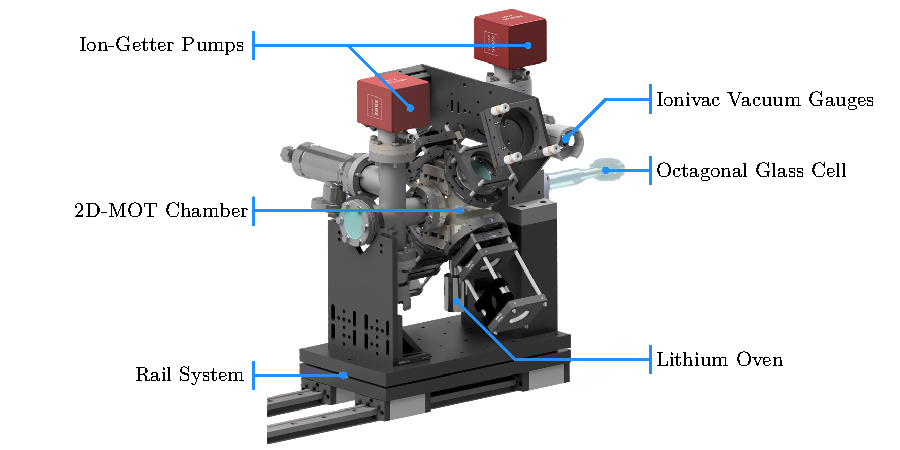
\includegraphics{fig-ai/setup.pdf} 
    \caption{
    \textbf{Rendering of the vacuum chamber setup.} 
    $^6$Li vapor emitted from the oven is captured and cooled by a 2D-MOT. A push beam transfers the pre-cooled atoms into the octagonal glass cell, where a 3D-MOT further cools and confines the atoms in all spatial directions, preparing them for subsequent loading into an ODT.
    }
    \label{fig:setup}
\end{figure}



The experimental apparatus is designed to realize and investigate complex quantum many-body dynamics using ultracold fermionic $^6$Li atoms. The primary objective of the setup is to create highly controllable initial quantum states, facilitate quantum simulation of the Fermi-Hubbard model, and enable precise measurements of quantum observables, such as entanglement entropy and particle correlations.

The experimental procedure starts with $^6$Li atoms emitted from an atomic oven. Lithium atoms are first collected and precooled in a two-dimensional magneto-optical trap (2D MOT), effectively capturing a high flux of atoms. From there, the atoms are transferred into a three-dimensional magneto-optical trap (3D MOT) for additional cooling and confinement, reaching temperatures near the Doppler limit (approximately 141~$\mu$K for $^6$Li) \cite{culemann_construction_2024, huang_construction_2024}.

Following the 3D MOT, atoms are loaded into a crossed optical dipole trap (ODT), generated by intersecting laser beams, creating a stable potential. At this stage, evaporative cooling further reduces the temperature significantly below quantum degeneracy conditions, reaching regimes where a molecular Bose-Einstein condensate (mBEC) can form. One of the first tasks within this thesis involved developing software for analyzing mBEC preparation data. Figure~\ref{fig:mbec} illustrates results from this analysis, demonstrating the phase space density (PSD) increasing with reduced temperature due to evaporative cooling (Fig.~\ref{fig:mbec}a). Measured atom density profiles at various temperatures show a characteristic bimodal distribution at low temperatures, indicative of mBEC formation (Fig.~\ref{fig:mbec}b). Fitting a Gaussian profile to the thermal wings of this distribution (red points in Fig.~\ref{fig:mbec}c) clearly reveals a central peak representing the condensed fraction (blue shaded area in Fig.~\ref{fig:mbec}c). While the generation of a molecular BEC is not part of the envisioned quantum simulation sequence, it impressively demonstrates the capabilities of the cooling and trapping system to reach quantum degeneracy.

\begin{figure}
    \centering
    \addletter{130}{a}
    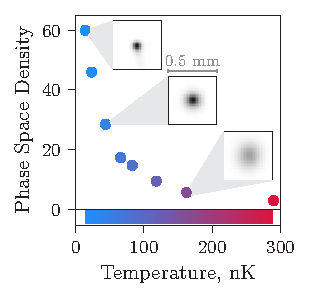
\includegraphics{fig-ai/m-bec-1-joined.pdf}
    \addletter{130}{b}
    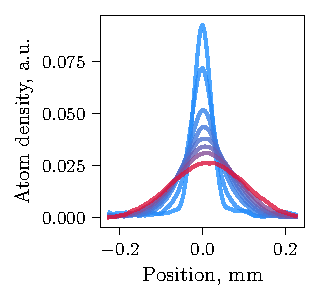
\includegraphics{fig-py/m-bec-2.pdf}
    \addletter{130}{c}
    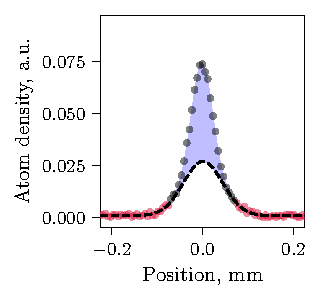
\includegraphics{fig-py/m-bec-3.pdf}
    \caption{
        \textbf{Molecular Bose-Einstein condensate data.}
        (a) Phase space density (PSD) increases as temperature decreases via evaporative cooling, indicating condensation onset. 
        (b) Measured atom density profiles normalized to unit area; color encodes temperature as in (a).
        (c) At low temperature, the profile shows a bimodal shape: a Gaussian fit to thermal wings (red dots) underestimates the central peak, revealing the mBEC component (blue area).
    }
    \label{fig:mbec}
\end{figure}



After reaching degeneracy in the ODT, atoms are adiabatically transferred into an optical tweezer array, implemented using crossed acousto-optic deflectors (AODs). These tweezers provide deterministic preparation of quantum states with single-site control, enabling initialization of specific many-body configurations essential for studying Fermi-Hubbard physics beyond thermal equilibrium. Precise atom number management is achieved through the spilling technique, which utilizes a magnetic field gradient and controlled reduction of tweezer depth to selectively retain atoms in low vibrational states \cite{culemann_construction_2024, huang_construction_2024}.

A critical aspect of our experiment is precise atom counting, particularly important when recapturing atoms from tweezers back into the MOT for calibration purposes. Atom number quantization can be clearly observed through fluorescence signal histograms, obtained with prolonged exposure times in a MOT loaded with a small number of atoms. Figure~\ref{fig:spillingadd}a shows discrete peaks corresponding to integer atom numbers, confirming accurate and reliable single-atom counting.

Future experimental plans involve transferring precisely prepared atoms into optical lattices engineered to simulate the Fermi-Hubbard model. The implemented lattice system features tunable geometry, capable of switching between square and triangular configurations without hardware modifications \cite{dux_optical_2023}. This flexibility enables systematic investigation of geometry-dependent phenomena in strongly correlated fermions. For vertical confinement, an accordion z-lattice provides the necessary two-dimensional character essential for Fermi-Hubbard physics while maintaining single-site resolution during imaging (detailed implementation described in \cite{huang_construction_2024}). Lattice depth and geometry, as well as disorder potentials, can be precisely tuned. Disorder is introduced using a digital micromirror device (DMD), enabling controlled studies of localization phenomena. 

To achieve single-site resolution with lattice spacings below the free-space imaging limit, a matter-wave magnifier (MWM) system is being implemented. Two additional harmonic trapping potentials have been installed for this purpose. The MWM coherently expands atomic distributions before imaging, enabling site-resolved detection in lattices with sub-micrometer spacing. Detailed theoretical and numerical analysis of the MWM system is presented in Section~\ref{sec:mwm}.

High-resolution, spin-resolved imaging is crucial for detailed characterization of quantum states in Fermi-Hubbard systems. The imaging system employs fluorescence-based free-space techniques, enabling rapid and high-fidelity spin detection with single-shot capability. Atoms are transferred to stretched hyperfine states, optimizing photon collection efficiency through closed cycling transitions. The implementation of spin-resolved detection represents a key development in this work. As part of this thesis, a complete distribution board for imaging and radiofrequency beam control was designed and assembled, including combining optics, acousto-optic modulator stages, and fiber coupling systems (detailed in Section~\ref{subsec:imaging-setup}). This enables simultaneous detection of both hyperfine ground states in a single experimental shot, providing direct access to local magnetization and spin correlations essential for characterizing magnetic phases in the Fermi-Hubbard model.

Control over atomic spin states is executed using dedicated radiofrequency (RF) and microwave (MW) antennas. The PCB-based RF antenna drives MHz-range spin transitions, while the MW loop antenna efficiently couples to hyperfine transitions, enabling coherent manipulation critical for state preparation, spin-selective procedures, and precise quantum control. These capabilities are essential for implementing spin-selective spilling protocols and preparing arbitrary spin-resolved configurations.

The entire experimental cycle (including state preparation, evolution, and measurement) is optimized for rapid repetition with a cycle time of approximately 2 seconds, allowing statistically robust data collection. The integration of all subsystems (from atomic source through deterministic state preparation to spin-resolved detection) provides a complete platform for investigating quantum many-body dynamics in engineered Fermi-Hubbard systems. The combination of programmable initial states, tunable Hamiltonians, and high-fidelity measurements enables systematic exploration of phenomena ranging from equilibrium quantum phases to out-of-equilibrium dynamics including thermalization and localization.




% !TEX root = ../master-thesis.tex

\begin{figure}[h!]
    \centering
    \addletter{85}{a} \phantom{4}
    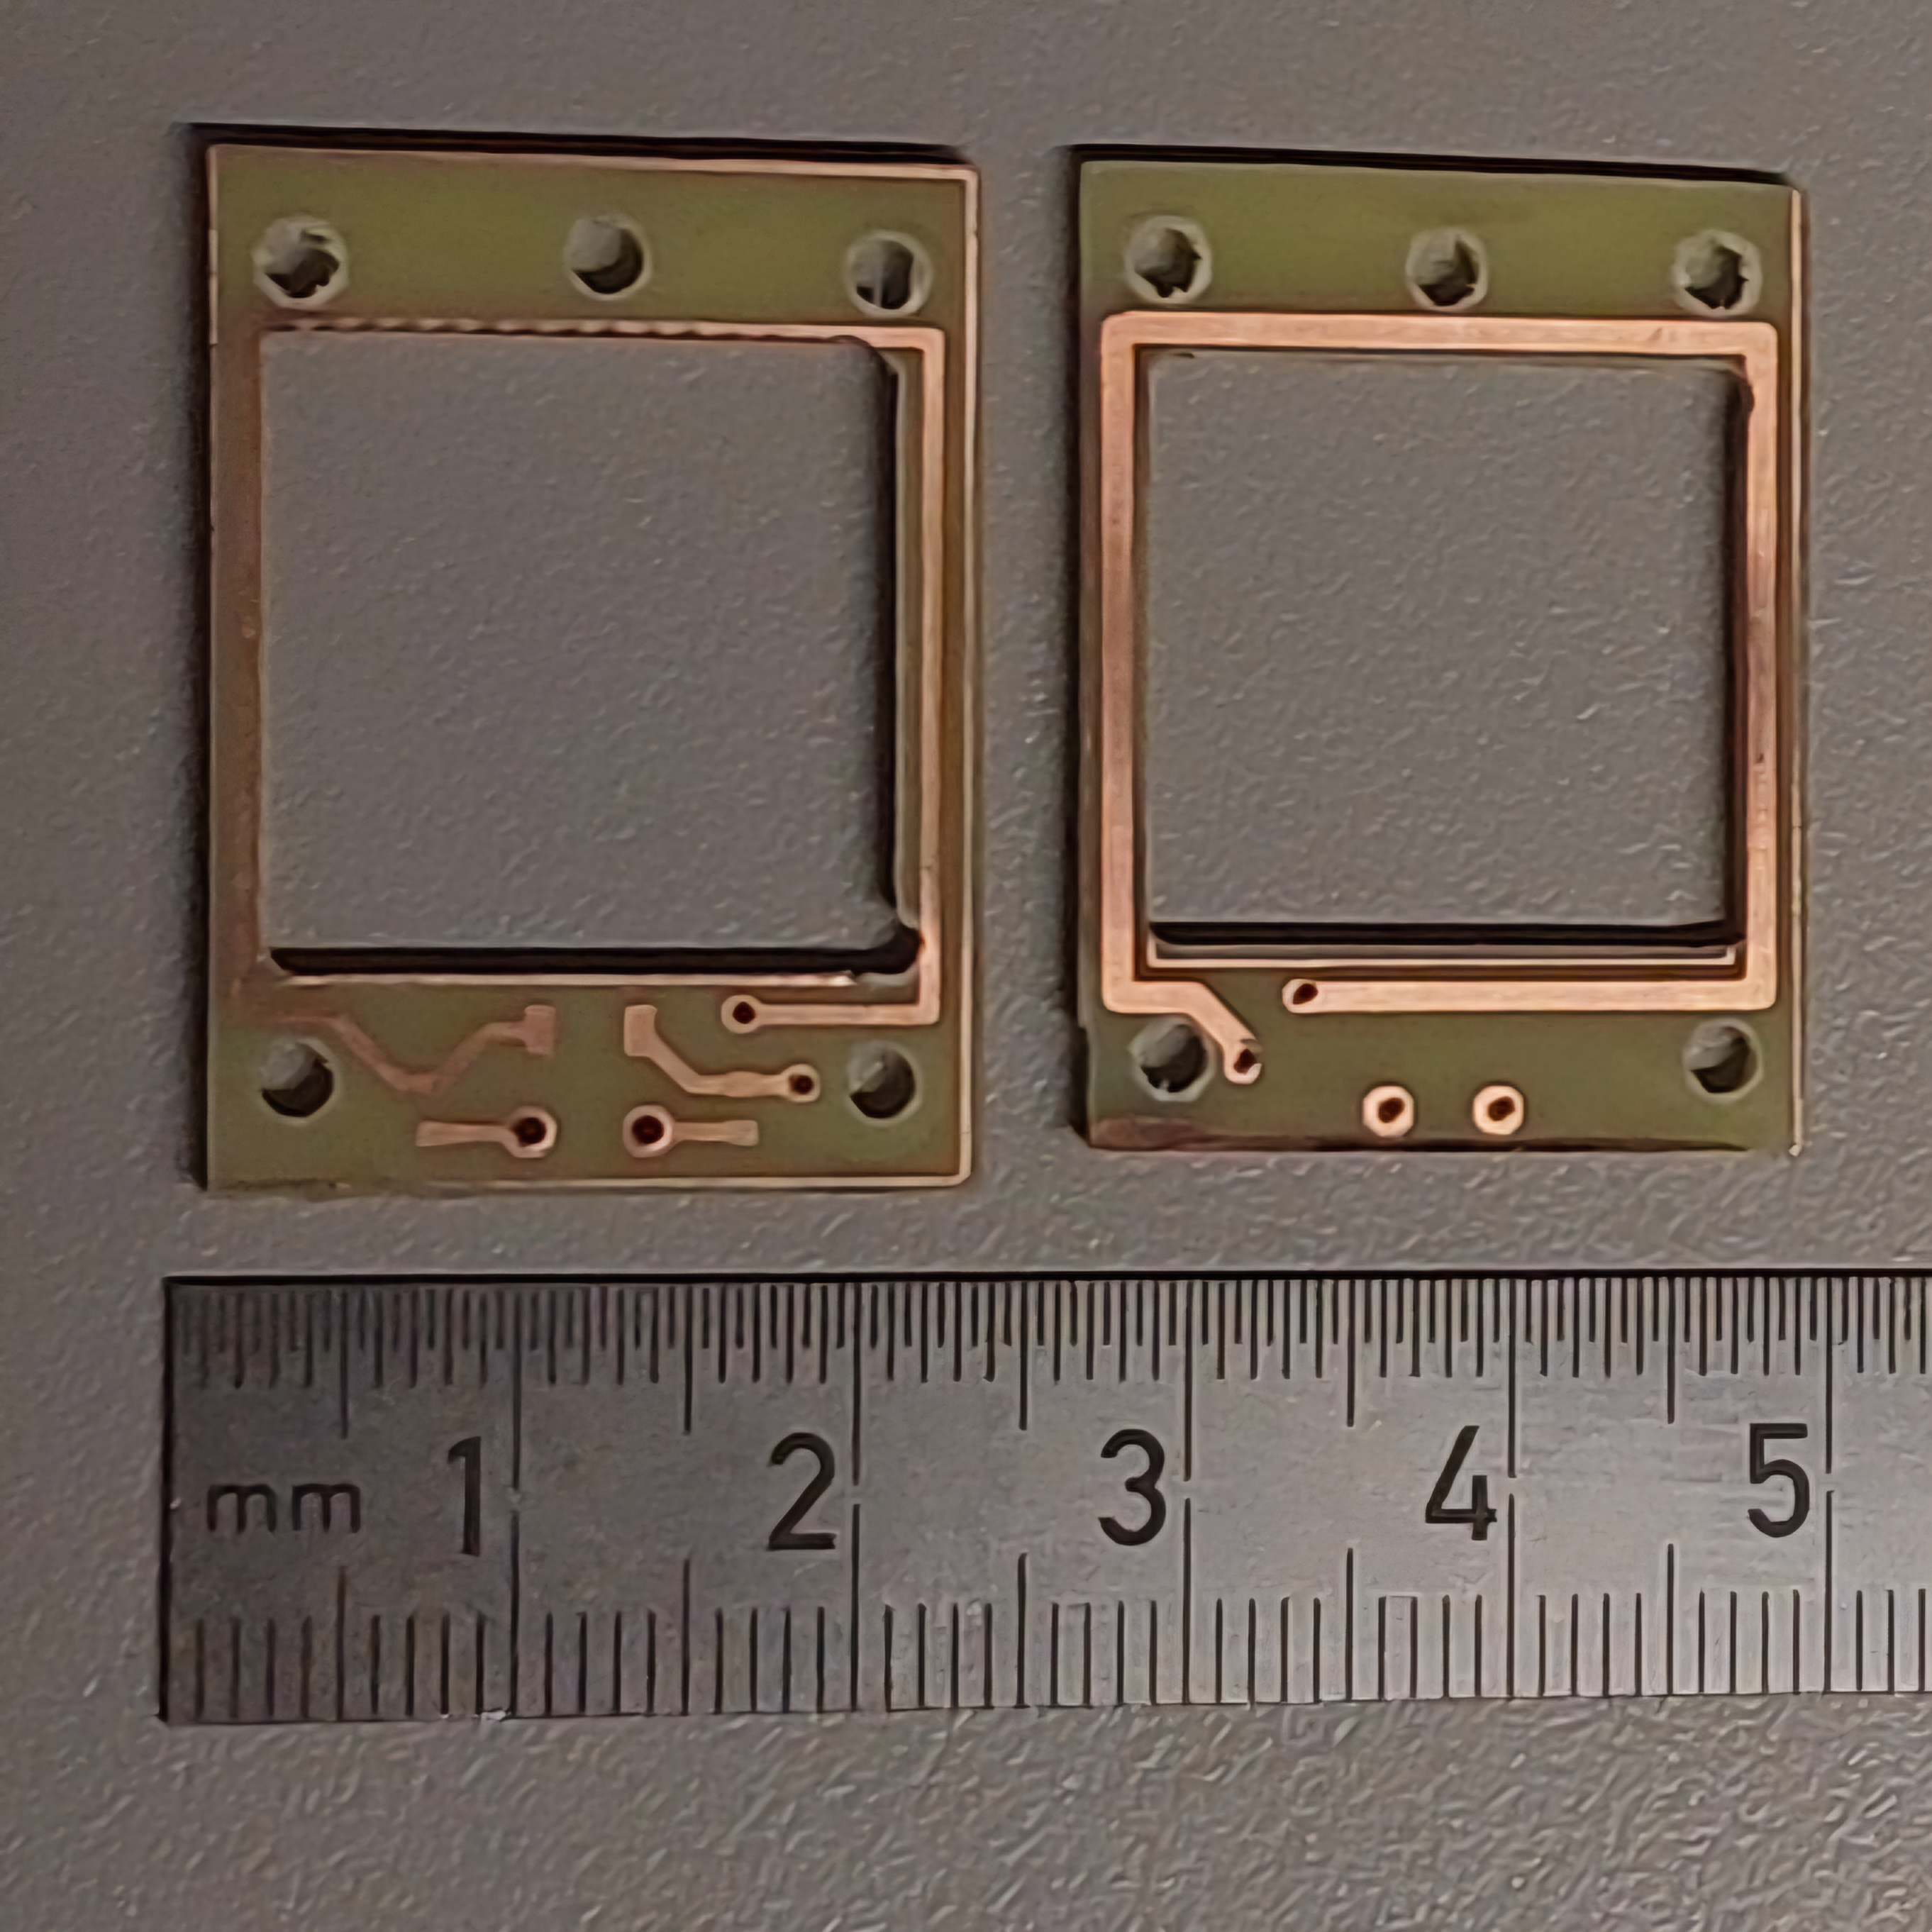
\includegraphics[width=1.25in]{imgs/RF.jpg}
    \hspace{1cm}
    \addletter{85}{b} \phantom{4}
    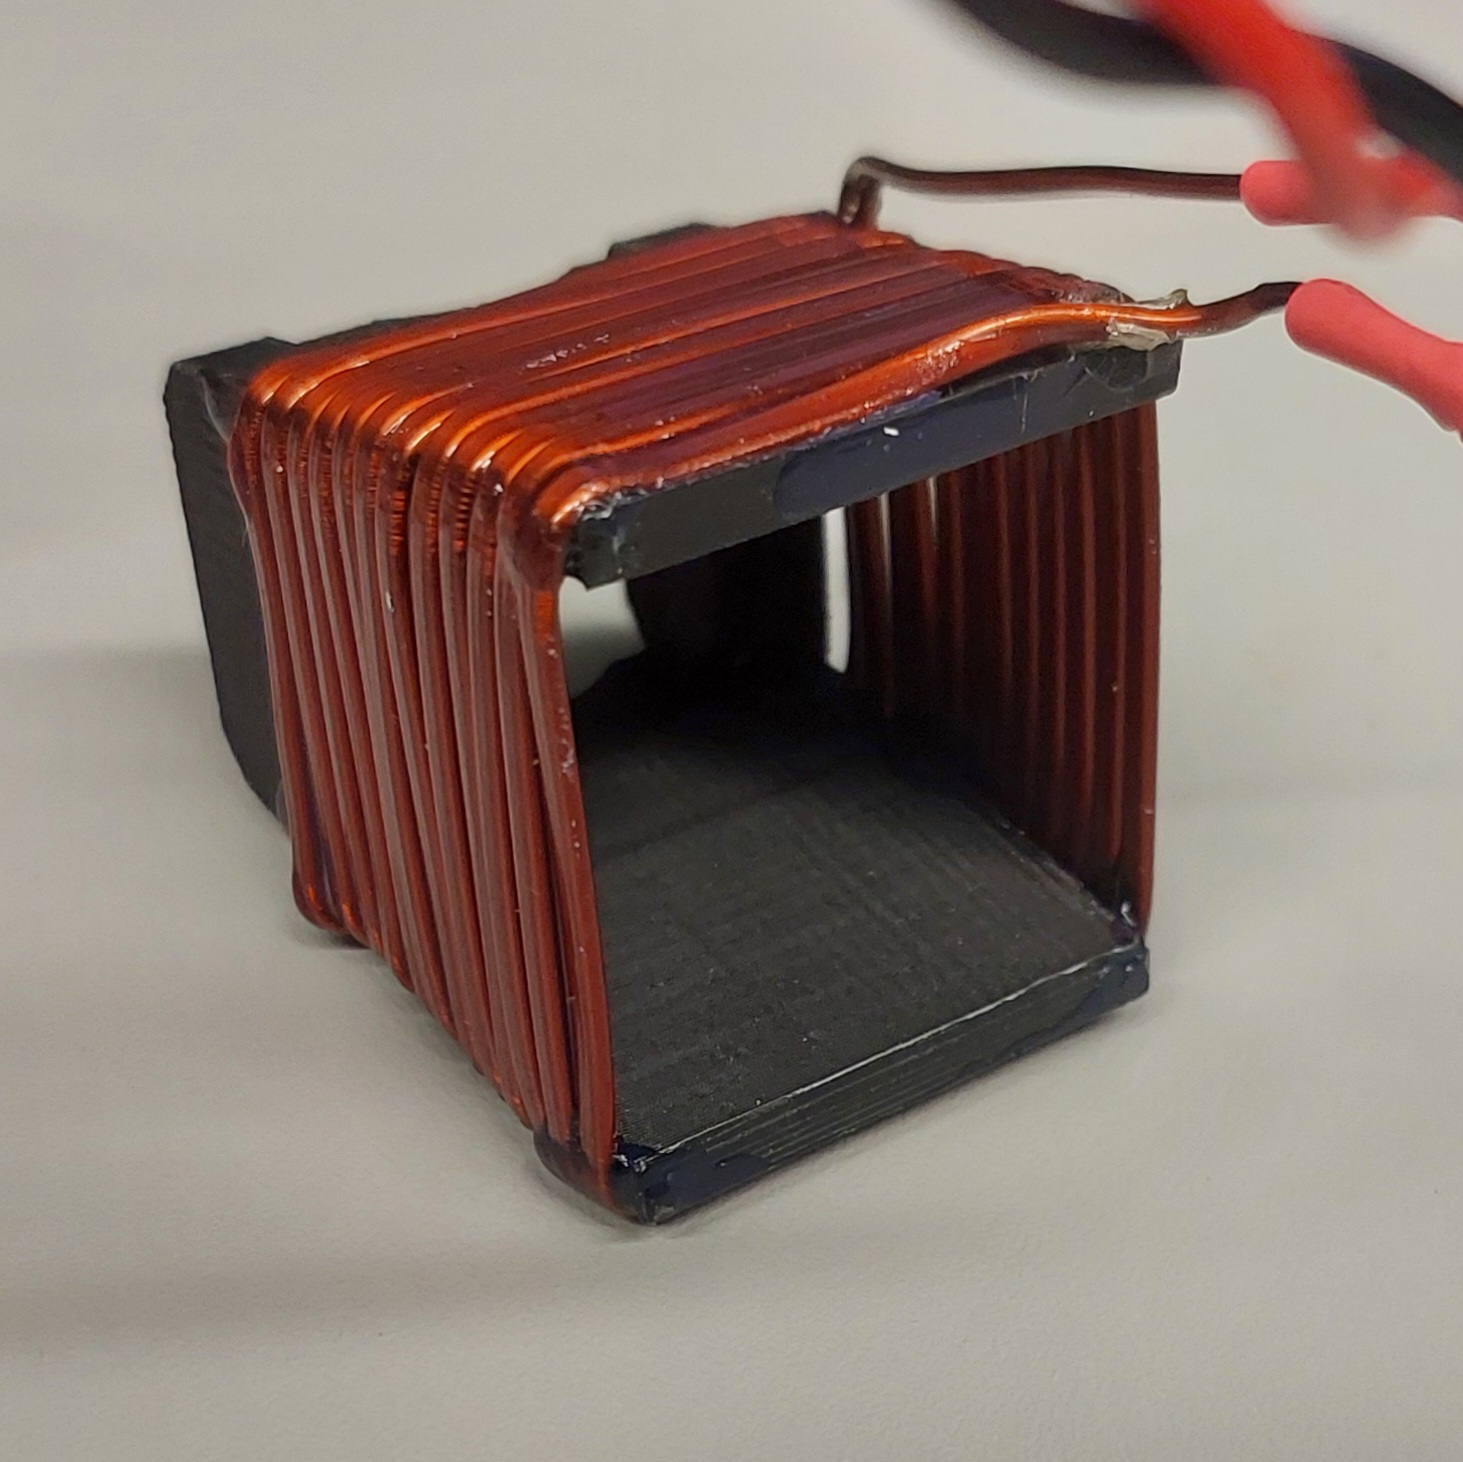
\includegraphics[width=1.25in]{imgs/MW.jpg}
    \caption{
        \textbf{RF and MW antennas used for spin control.}
        (a) PCB-based radiofrequency (RF) antenna used for driving spin transitions at MHz frequencies. 
        (b) Microwave (MW) loop antenna, designed to efficiently couple to hyperfine transitions in $^6$Li. 
        These antennas are used for coherent spin manipulation.
        % performance characterization via spin-flip fidelity is discussed in the following figures.
    }
    \label{fig:rfmw}
\end{figure}


\begin{figure}[h!]
    \centering
    \addletter{130}{a}
    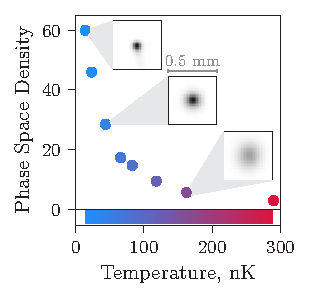
\includegraphics{fig-ai/m-bec-1-joined.pdf}
    \addletter{130}{b}
    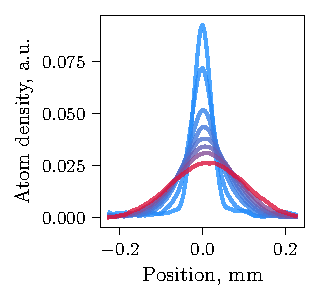
\includegraphics{fig-py/m-bec-2.pdf}
    \addletter{130}{c}
    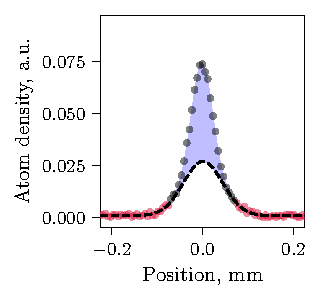
\includegraphics{fig-py/m-bec-3.pdf}
    \caption{
        \textbf{Molecular Bose-Einstein condensate data.}
        (a) Phase space density (PSD) increases as temperature decreases via evaporative cooling, indicating condensation onset. 
        (b) Atom density profiles normalized to unit area; color encodes temperature as in (a).
        (c) At low temperature, the profile shows a bimodal shape: a Gaussian fit to thermal wings (red dots) underestimates the central peak, revealing the mBEC component (blue area).
    }
    \label{fig:mbec}
\end{figure}




\begin{figure}[h!]
    \centering
    \addletter{145}{a}
    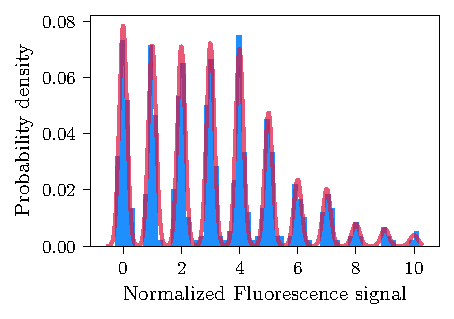
\includegraphics{fig-py/atom-counting.pdf}
    \phantom{4242}
    \addletter{145}{b}
    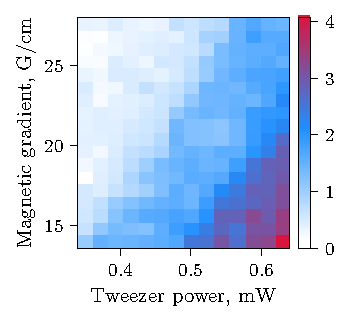
\includegraphics{fig-py/step-plot-2d.pdf}
    \caption{
        (a) Calibration histogram for single-atom counting based on fluorescence signal after after loading to the MOT. Clear quantized peaks correspond to integer atom numbers; the solid red line is a multi-Gaussian fit to the distribution. 
        (b) Measured 2D step plot as a function of tweezer power and magnetic field gradient. Each point indicates the average atom number obtained for a given combination of parameters. This map confirms that for any spill power, a suitable magnetic gradient can be found to achieve a desired quantized atom number.
    }
    \label{fig:spillingadd}
\end{figure}



\newpage
% --------------------------------------------------------------------------------------
\section{Single-atom spin-resolved free-space imaging} \label{sec:imaging}
% --------------------------------------------------------------------------------------

% Motivation and experimental approaches for spin-resolved imaging
\subsection{Introduction} \label{subsec:imaging-motivation} %  of Single-Atom Imaging Techniques
...

\subsection{\texorpdfstring{$^6$Li}{6Li} hyperfine structure and imaging scheme} \label{subsec:imaging-hyperfine}
% !TEX root = ../master-thesis.tex





\begin{figure}
    \centering
    \addletter{200}{a}
    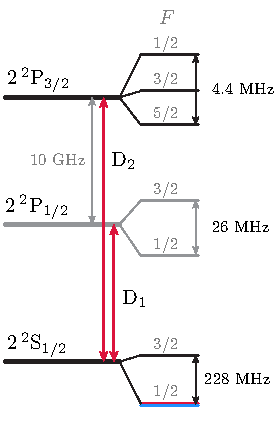
\includegraphics{fig-ai/li-levels-base.pdf}
    \hspace{1cm}
    \addletter{200}{b}
    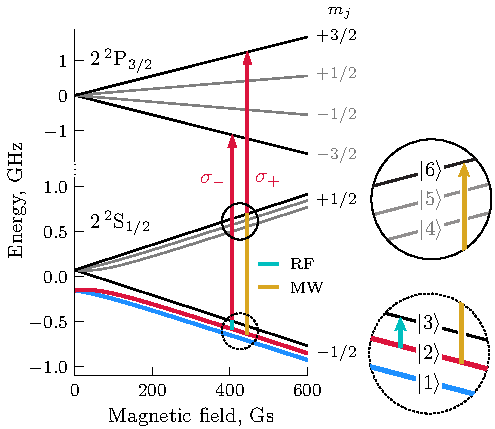
\includegraphics{fig-ai/li6-zeeman-broken-ai.pdf}
    \caption[${}^6$Li energy levels]{
        \textbf{${}^6$Li energy levels}. 
        a) Level diagram of the ground and excited states of ${}^6$Li \cite{gehm_preparation_2003}, including the D1 and D2 transitions around $\lambda = 671$~nm. 
        b) Zeeman splitting of the hyperfine levels of the $2\, {}^2\mathrm{S}_{1/2}$ and $2\, {}^2\mathrm{P}_{2/2}$ in ${}^6$Li \cite{serwane_deterministic_2011, sibalic_arc_2017}. As different spin states for physics we consider state $\ket{1}$ and $\ket{2}$, but for imaging it is worth to flip them to stretched states $\ket{6}$, $\ket{3}$. Colored lines indicate transitions driven by radiofrequency (RF) and microwave (MW) fields.
    }
    \label{fig:li6levels}
\end{figure}


% \subsection{$^6$Li hyperfine structure and imaging scheme}

The $^6$Li atom possesses a relatively simple electronic structure that makes it well-suited for quantum gas experiments. The electronic ground state $2\,^2\mathrm{S}_{1/2}$ exhibits hyperfine splitting due to the interaction between the electron and nuclear spins, resulting in two manifolds with total angular momentum $F = 1/2$ and $F = 3/2$ separated by 228 MHz (Fig.~\ref{fig:li6levels}a). The excited $2\,^2\mathrm{P}$ states relevant for optical transitions around $\lambda = 671$ nm include both the $\mathrm{P}_{1/2}$ (D$_1$ line) and $\mathrm{P}_{3/2}$ (D$_2$ line) levels \cite{gehm_preparation_2003}.

For quantum simulation experiments, the two lowest hyperfine states $|F = 1/2, m_F = \pm 1/2\rangle$, commonly denoted as $|1\rangle$ and $|2\rangle$, serve as the effective spin-1/2 system for realizing the Fermi-Hubbard model. These states exhibit favorable scattering properties and can be brought into resonant interaction using Feshbach resonances near accessible magnetic field strengths.

However, for fluorescence imaging, the stretched states $|3\rangle$ and $|6\rangle$ offer significant advantages over the $|1\rangle$ and $|2\rangle$ states. As shown in Fig.~\ref{fig:li6levels}b, at magnetic fields above $\sim 100$ G, the stretched states acquire nearly pure $m_J = \pm 1/2$ character due to Zeeman splitting \cite{serwane_deterministic_2011, sibalic_arc_2017}. This results in strong coupling to circularly polarized light: state $|3\rangle$ couples primarily to $\sigma^-$ transitions while $|6\rangle$ couples to $\sigma^+$ transitions. The stretched nature ensures closed cycling transitions with minimal population leakage to other hyperfine states, enabling efficient photon scattering rates exceeding those achievable with $|1\rangle$ and $|2\rangle$.

The imaging protocol therefore involves a preliminary step where atoms are transferred from the $|1\rangle$ and $|2\rangle$ physics states to the $|3\rangle$ and $|6\rangle$ imaging states using radiofrequency or microwave pulses. The polarization selectivity of the stretched states then enables spatial separation of the fluorescence signals using polarizing optics, as detailed in Section 3.4. This approach preserves the spin information while optimizing detection efficiency through the enhanced scattering cross-sections of the stretched states.

\subsection{SSH model} \label{subsec:imaging-ssh}
% !TEX root = ../master-thesis.tex



\begin{figure}
    \centering
    \addletter{140}{a}
    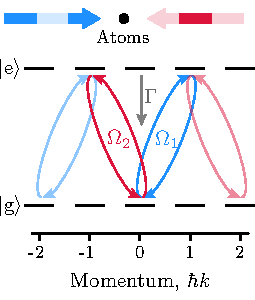
\includegraphics{fig-ai/ssh-scheme.pdf}
    \hfill
    \addletter{140}{b}
    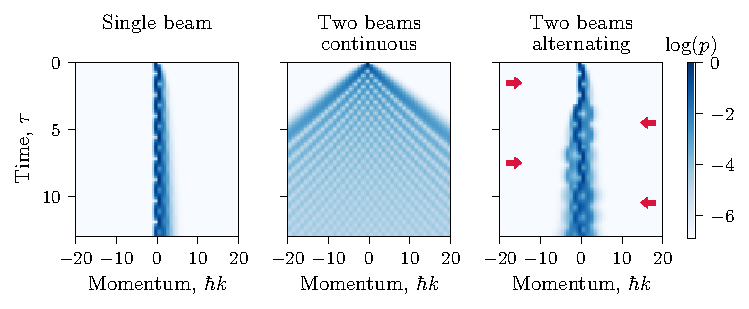
\includegraphics{fig-py/ssh-model.pdf}
    \caption{
        \textbf{Numerical simulation of momentum-space dynamics in the SSH model}. 
        a) Atoms undergo momentum-changing transitions via couplings $\Omega_1$ and $\Omega_2$, realizing a SSH-like quantum walk.
        b) Momentum distributions over time for different beam configurations: single beam (left) shows small shift; two continuous beams (middle) result in fast spreading; alternating beams (right) suppress spread.
    }
    \label{fig:sshmodel}
\end{figure}


Understanding the fundamental limitations and optimal strategies for free-space imaging requires a theoretical framework that captures the interplay between photon scattering, momentum transfer, and spatial resolution. This section develops a model based on the Su-Schrieffer-Heeger (SSH) Hamiltonian to explain the motivation for alternating beam sequences and to estimate the characteristic resolution limits of the imaging scheme.



\textbf{Recoil heating and momentum diffusion.} Although $^6$Li is a light atom and experiences relatively large momentum recoil during scattering, its broad D2 transition at $\lambda = 671$ nm allows for rapid photon emission. The typical recoil velocity is given by $v_\mathrm{rec} = h/(m\lambda)$, where $m$ is the atomic mass of $^6$Li and $\lambda$ is the wavelength of the imaging light. As the atom scatters photons at a rate $\Gamma$, each with random emission direction, it undergoes a random walk in momentum space, resulting in spatial diffusion during the imaging pulse.

The root-mean-square width of this random walk is approximately \cite{kruip_design_2024}
\begin{equation}
\sigma_\mathrm{rw} = \frac{1}{3} v_\mathrm{rec} \Gamma^{1/2} t^{3/2},
\label{eq:sigmarw}
\end{equation}
where $t$ is the total exposure time. For a fixed number of scattered photons $N_\mathrm{ph}$, we can express $t = N_\mathrm{ph}/\Gamma$, yielding
\begin{equation}
\sigma_\mathrm{rw} = \frac{1}{3} v_\mathrm{rec} \Gamma^{-1} N_\mathrm{ph}^{3/2}.
\end{equation}

This scaling highlights the trade-off between collecting more fluorescence photons and maintaining spatial resolution. In our system, with $N_\mathrm{ph} \approx 300$ scattered photons (of which approximately 10\% are detected by the camera), the resulting diffusion is on the scale of \red{10 $\mu$m}, which sets the practical limit for spatial resolution in free-space imaging of $^6$Li atoms.


\textbf{SSH model.} The scattering dynamics of a freely moving atom illuminated by resonant counter-propagating beams can be understood as a momentum-space quantum walk that maps onto the Su-Schrieffer-Heeger (SSH) model. In the standard SSH model, particles hop between two sublattices with alternating coupling strengths:
\begin{equation}
H = t_1 \sum_n |n,B\rangle \langle n,A| + t_2 \sum_n |n+1,A\rangle \langle n,B| + \text{h.c.}
\end{equation}

For the atomic case, this model takes the form:
\begin{equation}
H = \frac{\Omega_1}{2} \sum_p |p,g\rangle \langle p+1,e| + \frac{\Omega_2}{2} \sum_p |p-1,e\rangle \langle p,g| + \text{h.c.}
\end{equation}
where $\Omega_1$ and $\Omega_2$ correspond to the Rabi frequencies of the two counter-propagating beams, and $|p,g\rangle$ and $|p,e\rangle$ represent ground and excited states with momentum $p$.

A single beam produces systematic momentum transfer due to the finite linewidth $\Gamma$, leading to directed acceleration and displacement of the atomic cloud. When both beams are applied simultaneously, the atom undergoes coherent transitions between distant momentum states, resulting in rapid delocalization in space. This coherent coupling between momentum states separated by $2\hbar k$ leads to fast spreading of the momentum distribution.

The solution involves alternating the two beams rather than applying them simultaneously. This approach dramatically suppresses spatial diffusion by confining the coherent dynamics to simple oscillations between $\pm\hbar k$ states rather than allowing diffusion to higher momentum states. The evolution can be simulated by solving a Lindblad master equation:
\begin{equation}
i\hbar \partial_t \rho = [H(t), \rho] + \mathcal{L}[\rho],
\end{equation}
where $\mathcal{L}$ describes spontaneous emission. Numerical simulations demonstrate that alternating beam sequences significantly improve imaging fidelity compared to single-beam or simultaneous two-beam configurations (Fig.~\ref{fig:sshmodel}) as also was shown in \cite{su_fast_2025,bergschneider_spin-resolved_2018}.



The theoretical framework developed here provides the foundation for the experimental implementation described in the following sections, where the alternating beam protocol is realized using acousto-optic modulators. % SSH model as intuition

\subsection{Experimental setup} \label{subsec:imaging-setup}
\red{Здесь схема оптики для подготовки лучей в preparation board и схема лучей и подключения для main board}.

\begin{figure}
    \centering
    \addletter{140}{a}
    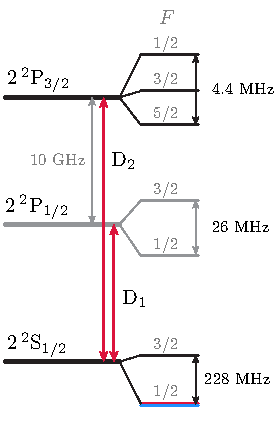
\includegraphics{fig-ai/li-levels-base.pdf}
    \hfill
    \addletter{140}{b}
    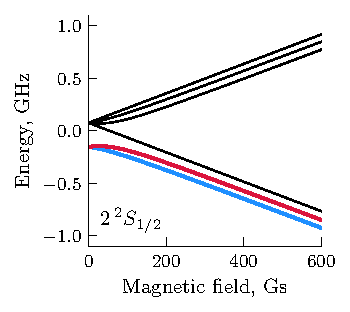
\includegraphics{fig-py/li6-zeeman.pdf}
    \hfill
    \addletter{140}{c}
    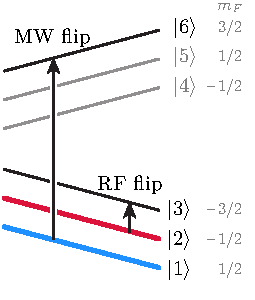
\includegraphics{fig-ai/li-levels.pdf}
    \caption{
        \textbf{${}^6$Li energy levels}. 
        a) Level diagram of the ground and 2P excited states of ${}^6$Li \cite{gehm_preparation_2003}. 
        b) Zeeman splitting of the hyperfine levels of the $2\, {}^2\mathrm{S}_{1/2}$ state in ${}^6$Li \cite{serwane_deterministic_2011, sibalic_arc_2017}. With dashed line was marked non-interacting regime for 1-2 mixture at 527 Gs. c) As different spin states for physics we consider state $\ket{1}$ and $\ket{2}$, but for imaging it is worth to flip them to close transitions.
        \red{Можно разделить (b), чтобы показать и расщепление для P32.}
    }
    \label{fig:li6levels}
\end{figure} % Optical scheme, atom preparation, probe configuration

\subsection{Image processing} \label{subsec:imaging-processing}
% !TEX root = ../master-thesis.tex


\begin{figure}
    \centering
    \addletter{125}{a}
    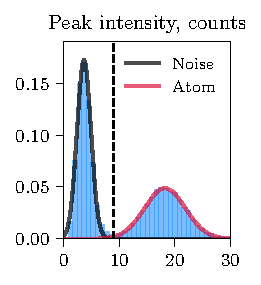
\includegraphics{fig-py/imaging-hist.pdf}
    \hfill
    \addletter{125}{b}
    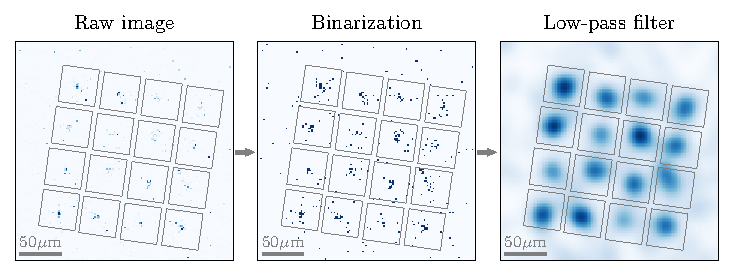
\includegraphics{fig-py/imaging-base.pdf}
    \caption[Single-atom identification and image processing]{
        \textbf{Single-atom identification and image processing.}
        a) Histogram of peak intensities extracted from binarized and low-pass filtered images shows a bimodal distribution: the first peak corresponds to camera noise (black), the second corresponds to single atoms (red). The dashed line indicates the threshold used for atom identification.
        b) Image processing pipeline: Raw fluorescence image (left), binarization by intensity thresholding (center), and application of a low-pass filter (right) to reveal spatially localized atomic signals. 
        % \red{Для (a) можно добавить fit, показав что иногда случаются и два атома.}
    }
    \label{fig:imaging}
\end{figure}

% \textbf{Camera and detection regime.}  
The imaging system uses a Nüvü HNü512 EMCCD camera, chosen for its high sensitivity and low noise in the few-photon regime. At $\lambda = 671$~nm, the sensor achieves a quantum efficiency (QE) of approximately 94\%~\cite{kruip_design_2024}. The camera is operated in photon counting mode with EM gain up to 5000, enabling single-atom detection from just tens of detected photons. During a typical imaging sequence, each atom emits around 300 photons, of which approximately 30 are detected on the camera after collection and transmission losses.

% \textbf{Binarization and filtering pipeline.}  
To mitigate the excess noise factor (ENF) inherent in EM amplification and to suppress clock-induced charges (CICs), we apply a binarization scheme. A fixed threshold (typically $5\sigma_\text{read}$ above the baseline noise) is used to convert raw images into binary maps, where each pixel is marked as "bright" if it exceeds the threshold and "dark" otherwise. This removes ambiguity due to the stochastic gain distribution and allows images to be treated as photon arrival maps.  

To reduce high-frequency noise while preserving localized atomic signals, we apply a Gaussian low-pass filter with a tunable width (typically $\sigma = 7$ px, close to the diffusion scale). This smooths the binarized images and helps identify spatially coherent clusters corresponding to single atoms. 
% \red{Optionally, a denoising step based on a circular neighbor-count kernel can be applied after binarization; see Appendix for implementation details.}

% \textbf{Atom identification from local maxima.}  
We locate candidate atom positions by searching for local maxima in the filtered images. Since the imaging beam is symmetric and atoms are spatially separated (due to the tweezer geometry), each atom forms a compact signal peak. To distinguish real atoms from CIC-induced noise clusters, we construct a histogram of peak amplitudes and apply a classification threshold based on the bimodal structure (see Fig.~\ref{fig:imaging}). This provides a robust method for single-atom detection within each image.

% \textbf{Use of ROI and regular array geometry.}  
During this work, all experiments were performed with a regular tweezer array. This allows us to restrict image analysis to known regions of interest (ROIs) around each expected atom location. This prior knowledge significantly simplifies the classification problem: we identify the atom at a given site as present or absent based on the presence of a peak in the corresponding ROI. This enables more reliable classification than in fully general imaging tasks as in \cite{bergschneider_spin-resolved_2018}.

% \textbf{Implementation and contribution.}  
The entire image analysis pipeline (bias correction, binarization, optional denoising, filtering, and classification) was implemented by the author in Python. The resulting code is vectorized and supports batch processing of image sequences. While the core concepts draw from existing methods developed in~\cite{bergschneider_spin-resolved_2018}, the current implementation is adapted to the geometry and noise characteristics of our setup. 
% Notably, the simplification due to known array geometry enables efficient and accurate analysis suitable for high-throughput acquisition.
 % Thresholding, noise filtering, spatial resolution

\subsection{Spin-resolved detection} \label{subsec:imaging-spin}
... % Two-step imaging, state identification, fidelity

\subsection{Spin manipulation} \label{subsec:imaging-flip}
% !TEX root = ../master-thesis.tex




% \textbf{Introduction and motivation.}
Manipulating the internal spin state of ultracold atoms is an essential element in quantum simulation experiments, particularly for us in context of deterministic state preparation and spin-resolved imaging.
Two widely employed methods for achieving controlled spin transitions in ultracold atomic systems are the Landau-Zener transition and coherent resonant $\pi$-pulse. The Landau-Zener approach involves adiabatically sweeping either the frequency of a driving field or the magnitude of a magnetic field across a spin-resonance. It has been widely applied due to its inherent robustness against small deviations in experimental parameters such as magnetic field fluctuations and frequency drifts. In contrast, the $\pi$-pulse method achieves spin flips by applying a resonant electromagnetic field pulse of precise duration, determined by the corresponding Rabi frequency. Although $\pi$-pulses offer considerably faster spin-flip operations, their fidelity is strongly sensitive to precise calibration of pulse duration, intensity, and frequency detuning, making them more susceptible to experimental noise and parameter instabilities.

Within the context of the current experiment, spin manipulation techniques serve two primary functions. Firstly, flipping atomic spins to stretched states enhances the efficiency of spin-resolved fluorescence imaging. Secondly, selective spin flips are integral to preparation protocols such as spin-selective spilling, allowing controlled removal of atoms in specific spin states. While the Landau-Zener method provided a practical starting point during initial setup stages (mainly due to its robustness against parameter variations) the progression toward faster experimental cycles motivated a transition towards using resonant $\pi$-pulses.

In the following paragraphs, the theoretical foundations of both Landau-Zener and $\pi$-pulse spin manipulation methods are described in detail. A comparative analysis then outlines their respective advantages and limitations in the presence of parameter noise, ultimately justifying the preferred choice adopted in this work.

\textbf{Landau-Zener transition.}
The Landau-Zener (LZ) transition \cite{landau_zur_1932,zener_non-adiabatic_1997} describes the non-adiabatic transition between two quantum states when the energy separation between these states is varied linearly in time. The Hamiltonian governing the dynamics of a two-level system undergoing such a process is expressed as:
\begin{equation}
H_{\text{LZ}}(t) = \frac{\hbar}{2}
\begin{pmatrix}
\Delta(t) & \Omega \\
\Omega & -\Delta(t)
\end{pmatrix},
\label{eq:LZ_Hamiltonian}
\end{equation}
where $\Delta(t)$ represents the instantaneous detuning between the system resonance and the external driving field, and $\Omega$ denotes the coupling strength (Rabi frequency) between the two states. Typically, the detuning is varied linearly as $\Delta(t) = \alpha t$, with $\alpha$ defined as the rate of change of detuning.

The transition probability $P_{\text{LZ}}$, derived analytically under the assumption of a linear sweep and constant coupling, is given by the Landau-Zener formula:
\begin{equation}
P_{\text{LZ}} = 1 - \exp\left(-\frac{\pi \Omega^2}{2\alpha}\right).
\label{eq:LZ_probability}
\end{equation}
This probability explicitly depends on the ratio of the squared coupling strength $\Omega^2$ to the detuning sweep rate $\alpha$. For slow sweeps ($\alpha \ll \Omega^2$), the system achieves near-complete transitions ($P_{\text{LZ}}\rightarrow1$), whereas faster sweeps reduce the fidelity (see Fig.~\ref{fig:spin-flip}b).

An important experimental advantage of the Landau-Zener method is its robustness against fluctuations in experimental parameters, such as variations in the magnetic field or the driving frequency. Small deviations in magnetic field gradients or frequency drifts typically have minimal impact on transition fidelity due to the exponential character of Eq.~\eqref{eq:LZ_probability}. This robustness is particularly valuable in experiments where shot-to-shot variations in magnetic fields are inevitable. Despite its robustness, the Landau-Zener transition requires relatively long timescales ($t_{\text{LZ}} \gg 1/\Omega$) to achieve high transition fidelities, which can slow down experimental cycles and increase exposure to decoherence processes.

\textbf{Rabi $\pi$-pulse.}
An alternative technique for coherent spin manipulation is the resonant Rabi oscillation method, commonly known as the $\pi$-pulse approach. This method exploits coherent driving of the transition between two spin states at constant resonance, enabling deterministic and rapid population transfer.

The dynamics under resonant excitation are described by the Hamiltonian in Eq.~\eqref{eq:LZ_Hamiltonian} with a constant detuning $\Delta=\text{const}$. By applying a resonant driving field ($\Delta=0$) for the duration $t_\pi = \pi/\Omega$, the system achieves complete inversion of the spin populations, thus realizing an ideal spin-flip operation between states $\ket{1}$ and $\ket{2}$.

The primary advantage of the $\pi$-pulse technique is its speed: the required pulse duration is significantly shorter than that for Landau-Zener sweeps ($t_\pi \ll t_{\text{LZ}}$), as evidenced by rapid Rabi oscillations in Fig.~\ref{fig:spin-flip}c. However, the fidelity of $\pi$-pulse transitions is highly sensitive to deviations from the exact resonance condition ($\delta \neq 0$), as well as inaccuracies in pulse duration and field amplitude. This sensitivity is captured analytically by the generalized Rabi oscillation formula:
\begin{equation}
P_{\pi} = \frac{\Omega^2}{\Omega^2+\delta^2}\sin^2\left(\frac{\sqrt{\Omega^2+\delta^2}}{2}t_{\pi}\right).
\label{eq:pi_fidelity}
\end{equation}

Shot-to-shot fluctuations, especially those in the magnetic field, directly translate into variations in resonance conditions and consequently introduce systematic and random errors in spin-flip fidelity. As a result, consistently high fidelity using $\pi$-pulses necessitates stringent experimental stabilization of magnetic fields, pulse timing, and amplitude calibration.


\begin{figure}
    \centering
    \addletter{105}{a}
    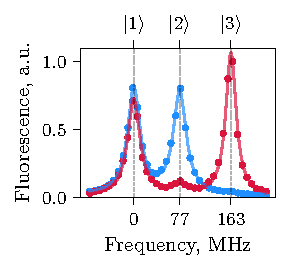
\includegraphics{fig-py/spin-flip-1.pdf}  \phantom{4}
    \addletter{105}{b}
    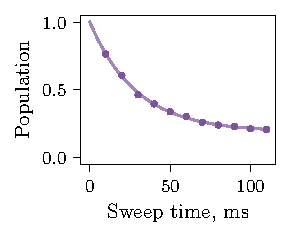
\includegraphics{fig-py/spin-flip-2.pdf}  \phantom{4}
    \addletter{105}{c}
    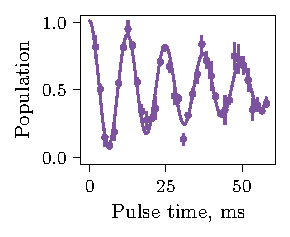
\includegraphics{fig-py/spin-flip-3.pdf}  \phantom{4}
    \caption[Characterization of spin manipulation protocols]{
        \textbf{Characterization of spin manipulation protocols.}
        (a) Fluorescence signal measured in the ODT before (blue) and after (red) applying a Landau-Zener sweep between states $\ket{2}$ and $\ket{3}$, showing population transfer to the target state. 
        (b) Final population in $\ket{2}$ as a function of sweep duration, consistent with the Landau-Zener model. 
        (c) Rabi oscillations observed when applying resonant RF $\pi$-pulse between states $\ket{2}$ and $\ket{3}$, demonstrating coherent control of the spin transition.
    }
    \label{fig:spin-flip}
\end{figure}


% \textbf{In this experiment.}
In the present experiment, spin-state populations are routinely measured by scanning the laser frequency while simultaneously recording the fluorescence signal of atoms either confined in the ODT or directly in optical tweezers. Figure~\ref{fig:spin-flip}a demonstrates a typical example, showing clear fluorescence peaks corresponding to distinct spin states. Such spectral scans provide a reliable quantitative method for assessing the efficiency of spin-state transitions.
% 
Initially, spin manipulation in this experiment relied primarily on Landau-Zener sweeps. 
% Operating at moderate coupling strengths ($\Omega \sim 1~\text{kHz}$), transition fidelities around \red{95\%} were achieved. 
Subsequent technical improvements in the RF and MW antenna designs allowed increasing the effective coupling strength up to approximately 10~kHz. Employing $\pi$-pulses at this higher coupling strength consistently yielded fidelities of \red{99\%}.

In conclusion, while Landau-Zener sweeps provided a robust and convenient method for spin-state manipulation during initial setup phases, the improvements in RF/MW coupling strengths ultimately favored the adoption of faster and more efficient $\pi$-pulse protocols.

\subsection{Conclusion} \label{subsec:imaging-conclusion}
% !TEX root = ../master-thesis.tex

This section has detailed the implementation of a spin-resolved free-space imaging system for ${}^6$Li atoms in an optical tweezer array. The approach is tailored to fast-cycle experiments and leverages the intrinsic spacing of the array to bypass the need for sub-micron spatial resolution. 
% 
The free-space fluorescence method was motivated both conceptually and practically, with an emphasis on momentum-space dynamics during imaging. Theoretical considerations based on the SSH model support the use of alternating beam sequences to reduce spatial diffusion, thereby improving localization fidelity.

The optical setup includes two independent laser beams driving stretched-state cycling transitions, with modulation handled via AOMs and synchronized control electronics. A distribution board was constructed to combine and route the beams, ensuring symmetric delivery to the atoms. 
% 
The image analysis pipeline applies binarization and spatial filtering to extract single-atom signals from low-flux data. The use of fixed array geometry enables simplified region-of-interest (ROI) analysis and improves classification reliability. All components of the processing chain are implemented in a parallelized, vectorized framework to support high-throughput acquisition.

Spin information is extracted by mapping fluorescence from $\sigma^+$ and $\sigma^-$ transitions to distinct regions on the camera. A per-site classification algorithm assigns spin states based on signal strengths in these regions. Validation against calibrated single-atom counted experiments yields a classification accuracy of approximately 99\% under typical experimental conditions.
% 
These techniques constitute a fast and reliable imaging solution suitable for experiments requiring spin-resolved readout, and are readily extensible to future array sizes and imaging geometries.



\newpage
% --------------------------------------------------------------------------------------
\section{Tweezer array system} \label{sec:tweezer}
% --------------------------------------------------------------------------------------

\subsection{Introduction} \label{subsec:state-prepation-overview}
% !TEX root = ../master-thesis.tex


\begin{figure}
    \centering
    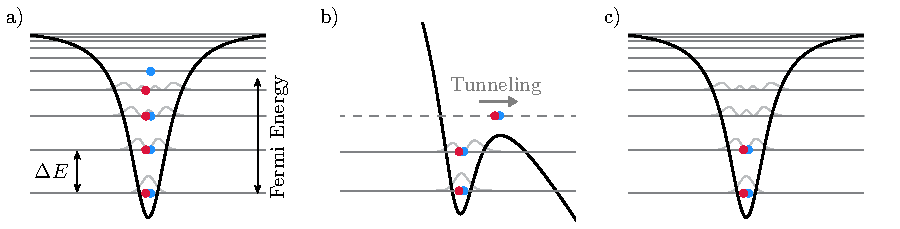
\includegraphics{fig-ai/preparation.pdf}
    \caption[Deterministic preparation via spilling]{
        \textbf{Deterministic preparation via spilling.}
        (a) Fermionic atoms are initially loaded into a tightly confined optical tweezer, forming a Fermi sea occupying the approximately 1D harmonic oscillator levels up to the Fermi energy. 
        (b) A magnetic field gradient tilts the potential, and the trap depth is lowered such that atoms above a defined spill level tunnel out. 
        (c) This procedure leaves a well-defined number of atoms in the lowest energy states, with a preparation fidelity of approximately 95\%. 
        Blue and red dots denote atoms in different spin states; gray curves indicate the bound-state wavefunctions.
    }
    \label{fig:preparation}
\end{figure}


Quantum simulation of strongly correlated many-body systems requires precise control over initial quantum states to access regimes beyond thermal equilibrium and investigate specific quantum phenomena. The ability to prepare designer initial states with single-site and single-spin resolution has become essential for studying complex quantum phases, far-from-equilibrium dynamics, and engineered many-body Hamiltonians. Beyond fundamental many-body physics, deterministic state preparation is crucial for quantum chemistry simulations~\cite{gkritsis_simulating_2025}, and for broader fermionic quantum computing applications~\cite{gonzalez-cuadra_fermionic_2023}.
% This capability is particularly important for distinguishing between different dynamical regimes, such as many-body localization (MBL) and Anderson localization, where the initial state configuration directly influences the observable signatures and relaxation dynamics.

Traditional approaches for loading atoms into optical lattices rely on transferring atomic clouds from magneto-optical traps (MOTs) or optical dipole traps (ODTs) into the periodic potential created by interfering laser beams. While these methods have enabled significant progress in quantum simulation, they face fundamental limitations in state preparation flexibility. The primary constraint arises from the lack of sufficiently different spin-dependent potentials that would enable site-selective manipulation of internal atomic degrees of freedom. Although spatial light modulators (SLMs) and digital micromirror devices (DMDs) can create programmable optical potentials for compensating harmonic confinement and achieving uniform filling~\cite{mazurenko_cold-atom_2017}, the construction of arbitrary spin-resolved configurations remains challenging with conventional lattice-loading techniques.

Optical tweezers have also been employed to enhance conventional thermal loading approaches through site-resolved addressing. Notable implementations include using individual tweezers to locally increase the potential depth during lattice loading, thereby creating controlled defects in otherwise uniformly filled systems~\cite{koepsell_imaging_2019}. Such hybrid approaches have enabled studies of antiferromagnetic order with engineered impurities.
% , starting from near-Mott insulating conditions at temperatures around $0.45t$ with interaction strength $U/t = 14$. 
However, these methods still rely fundamentally on thermal equilibration and are limited in their ability to construct arbitrary initial configurations.

The emergence of optical tweezer arrays has provided a transformative solution to these state preparation challenges through deterministic, bottom-up assembly of many-body quantum systems~\cite{serwane_deterministic_2011}. Unlike traditional loading approaches that rely on statistical distributions, tweezer-based methods enable constructive control over both spatial and internal degrees of freedom. Early demonstrations showed the feasibility of deterministic few-body preparation in one-dimensional systems, with achieved fidelities of approximately 95\% for doublon preparation~\cite{holten_pauli_2022,spar_realization_2022}. Recent advances have extended these capabilities to one-dimensional tweeyer arrays~\cite{stuart_single-atom_2018,gyger_continuous_2024,spar_realization_2022}.

The core principle underlying tweezer-based state preparation involves the spilling technique, which exploits the quantized energy levels of fermions in tightly confined optical potentials. By adiabatically reducing the trap depth while applying magnetic field gradients, atoms occupying higher energy levels become unbound and escape, while those in lower levels remain trapped. The differential magnetic moments of hyperfine ground states enable spin-selective spilling: at specific magnetic field strengths, only one spin component experiences significant forces from applied gradients, allowing deterministic preparation of sites containing empty, single spin-up, single spin-down, or spin-paired configurations.

As part of this work, a tweezer array system was developed based on crossed acousto-optic deflectors (AODs), enabling spin-selective two-dimensional individual site control. The system aims deterministic preparation of arbitrary spin- and site-resolved occupation patterns through a sequence of global and spin-selective spilling operations. Current preparation fidelities reach 81\% for doublon preparation, with identified improvements in magnetic field stabilization expected to approach the 95\% benchmarks demonstrated in other laboratories~\cite{holten_pauli_2022,serwane_deterministic_2011,spar_realization_2022}.

To the best of our knowledge, arbitrary spin-selective state preparation in two-dimensional fermionic systems has not been previously demonstrated. 
% This capability represents a significant advancement for investigating dynamics of different Hamiltonians and implementing quantum chemistry simulations~\cite{gkritsis_simulating_2025}. 
The achievement of programmable spin-selective filling constitutes one of the central results of this work. Despite currently modest fidelities, the proposed methods appear promising for future developments in quantum simulation of strongly correlated fermions.

The integration of deterministic state preparation with the spin-resolved imaging capabilities described in Section~\ref{sec:imaging} provides the experimental tools necessary for systematic investigation of quantum many-body dynamics. The ability to prepare specific initial configurations and measure their subsequent evolution with single-site, single-shot resolution enables direct study of phenomena such as quantum thermalization and localization. 
% As demonstrated through numerical simulations in Section~\ref{sec:fhmodel}, the distinction between MBL and Anderson localisation dynamical regimes depends on both the initial state preparation and the measurement of local observables including density profiles, magnetization patterns, and correlation functions.

This chapter presents the design, implementation, and characterization of the complete tweezer array system. Section~\ref{subsec:aodconcept} describes the optical setup and acousto-optic deflector control systems. Section~\ref{subsec:control} details the calibration procedures for achieving uniform tweezer arrays and precise depth control. Section~\ref{subsec:state-prepation} presents the spilling protocols for deterministic few-body preparation. Section~\ref{subsec:spin-selective-spilling} introduces the spin-selective manipulation techniques enabling arbitrary spin-resolved configurations. Section~\ref{subsec:arbitrary-occupation-loading} demonstrates the complete sequence for preparing complex many-body initial states. The developed platform provides a foundation for future quantum simulation experiments investigating strongly correlated fermions in engineered two-dimensional systems.

\subsection{Acousto-optic deflector} \label{subsec:aodconcept}

Optical tweezer arrays provide a flexible platform for preparing ultracold atomic systems with site-resolved control. By trapping individual atoms in focused laser beams, it becomes possible to initialize many-body states with controlled geometry, low entropy, and tunable local parameters.

In our setup, a two-dimensional array of tweezers is created using two orthogonal acousto-optic deflectors (AODs). Each AOD diffracts multiple beams along one axis, and their intersection forms the full array. The resulting intensity at site $(i,j)$ factorizes as $P_{ij} = H_i V_j$, where $H_i$ and $V_j$ are set by the drive amplitudes applied to each AOD. This structure simplifies calibration and allows fast control of the entire array using a small number of parameters.

Compared to holographic or lattice-based approaches, the AOD system offers rapid reconfigurability and independent control of individual traps. This enables preparation of custom spin and density patterns, as well as dynamic manipulation during the experimental sequence. Such capabilities are useful, for example, for initializing specific configurations, removing defects, or performing spatially selective operations before loading atoms into an optical lattice for further evolution.

\textbf{AOD operation.} Each AOD consists of a crystal driven by a piezoelectric transducer. An incoming laser beam $(\vc{k}_{\mathrm{in}}, \omega_{\mathrm{in}})$ interacts with the induced acoustic wave $(\vc{q}, \Omega)$ via Bragg diffraction, producing an outgoing beam $(\vc{k}_{\mathrm{out}}, \omega_{\mathrm{out}})$:
\begin{equation*}
    \vc{k}_{\mathrm{out}} = \vc{k}_{\mathrm{in}} + \vc{q}, \qquad \omega_{\mathrm{out}} = \omega_{\mathrm{in}} + \Omega.
\end{equation*}
The frequency $\Omega$ determines the deflection angle $\theta$ through the Bragg condition, while the amplitude of the RF signal controls the diffracted optical power. Each RF tone can be described by a triple $(\Omega_j, a_j, \varphi_j)$, corresponding to its frequency, amplitude, and phase. Applying a set of such tones to an AOD results in a superposition of multiple diffracted beams, with the amplitude $a_j$ determining the power in each beam and the phase $\varphi_j$ influencing their relative coherence.


\textbf{Factorized intensity distribution.} 
To create 2D arrays, we combine two AODs oriented along orthogonal axes (fig.~\ref{fig:control}a), as described in~\cite{culemann_construction_2024}.
Each axis is driven by a set of RF tones. In the paraxial approximation, the resulting 2D intensity pattern can be written as a rank-1 product of two vectors:
\begin{equation*}
    P_{ij} = H_i V_j,
\end{equation*}
where $H_i$ and $V_j$ correspond to the powers of individual beams generated by the horizontal and vertical AOD, respectively. The factorization of the output power can be verified via:
\begin{equation}
\label{eq:factorisability}
    P \overset{\mathrm{SVD}}{=} \textstyle \sum_r \Lambda_r \vc{H}_r \vc{V}_r\T,
    \hspace{10 mm} 
    \text{factorisability} = \Lambda_0 / \sum_r \Lambda_r 
\end{equation}
which provides a natural measure of factorization. For arrays ranging from $2\times2$ to $10\times10$, the factorisability measure $\Lambda_0 / \sum_r \Lambda_r$ is consistently above $0.99$. For the $4\times4$ array used in most of our experiments, we obtain a typical value of $0.997(1)$.

\textbf{Tweezer array control.} The tweezer output beam powers are nonlinear functions of the input amplitudes $\vc{a}$:
\begin{equation}
    \label{eq:taylerexp}
    P_j = F_j(\vc{a}) = \cancel{F_j(\vc{0})} + F'_{ji} a_i + \tfrac{1}{2} F''_{j i_1 i_2} a_{i_1} a_{i_2} + \ldots
\end{equation}
The goal is to control\footnote{
    For amplitudes in the range $a_i \in [0.7, 1.0]$, we find that a linear or quadratic approximation suffices. In practice, we reconstruct the Jacobian matrix $F'_{ji}$ using camera-based calibration, as discussed in Sec.~\ref{subsec:control}.
} the full matrix $P_{ij}$ using only two sets of parameters: horizontal amplitudes $\vc{h}$ and vertical amplitudes $\vc{v}$. 

It will later be necessary to reconstruct $(H_i, V_j)$ from measured intensity distribution $P_{ij}$, so it is convenient to choose a factorized model $P_{ij} = \Lambda H_i V_j$, with the normalization:
\begin{equation*}
    \sum_i H_i = \sum_j V_j = 1, \hspace{5 mm} \sum_{ij} P_{ij} = \Lambda.
\end{equation*}
This allows for an explicit decomposition:
\begin{equation}
    \textstyle
    \frac{1}{\Lambda} \sum_j P_{ij} = H_i \sum_j V_j = H_i,
    \hspace{5 mm} 
    \frac{1}{\Lambda} \sum_i P_{ij} = V_j \sum_i H_i = V_j,
    \hspace{5 mm} 
    \sum_{ij} P_{ij} = \Lambda,
    \label{uv-decomposition}
\end{equation}
which is fully equivalent to a rank-1 SVD of $P_{ij}$.

It is worth noting that, as shown in Fig.~\ref{fig:control}d, the total scale parameter $\Lambda$ defined in this way is proportional to the total input amplitude, $\sub{a}{sum} = \sum_j h_j + \sum_j v_j$. This effectively decouples local balancing from global power constraints, simplifying the control problem.

% \grey{This allows us to adjust the global scale $\Lambda$ (via a shared AOM or pre-AOD attenuation) and balance individual amplitudes using only two $n$-dimensional vectors.}
 % Tweezer arrays as control tool, overview

\subsection{Optical setup}
...


% \textbf{Acousto Optic Deflector (AOD)}. AOD, как и AOM, состоит из кристалла, который модулируется пьезоэлементом. Проходящие через кристалл фотоны $(\sub{\vc{k}}{in}, \sub{\omega}{in})$ рассеиваются на фононах $(\vc{q}, \Omega)$ via Bragg diffraction. To have higher efficiency we need to satisfy Bragg condition (проверить и добавить источник)
% \begin{equation*}
% 	\sub{n}{sc} q = \sub{k}{in} \sin(\theta),
% \end{equation*}
% \grey{где $\theta$ это угол между $\vc{k}$ и нормалью к $\vc{q}$} \red{(добавить рисунок)}. Внутри AOD находится несколько пьезоэлементов, к которым ведут провода подобранной длины так, чтобы при изменение частоты $\Omega$ направление $\vc{q}$ менялось соответсвующим Bragg condition образом. Это помогает улучшить диффракционную эффективность \grey{(добавить определение или ссылку)} AOD. На выходе полуются $(\sub{\vc{k}}{out}, \sub{\omega}{out}) = (\sub{\vc{k}}{in}+\vc{q}, \sub{\omega}{in} + \Omega)$. 
% Имея набор частот в модулирующем сигнале $(\vc{q}_j, \Omega_j)$ получим на выходе набор лучей
% \begin{equation*}
% 	(p_j, \vc{k}_j, \omega_j) = (F_j(\vc{a}, \sub{\vc{\omega}}{in}), \sub{\vc{k}}{in}+\vc{q}_j, \sub{\omega}{in} + \Omega_j),
% \end{equation*}
% c мощностью в каждом луче на выходе $p_j$. Регулируя вектор амплитуд $\vc{a}$, подающихся в AOD можно контролировать выходную мощность $\vc{p}$. 
 % AODs, array generation, optical layout

\subsection{State preparation} \label{subsec:state-prepation}
% !TEX root = ../master-thesis.tex

% Тут хочется добавить общую последовательность эксперимента. То есть если говорю про imaging with flashing, добавим что происходит с магнитным полем и прочим важным (спросить Намана). Аналогично для state preparation, imaging.

% m: 40-42, 67-70
% h: 84-86, 


\begin{figure}
    \centering
    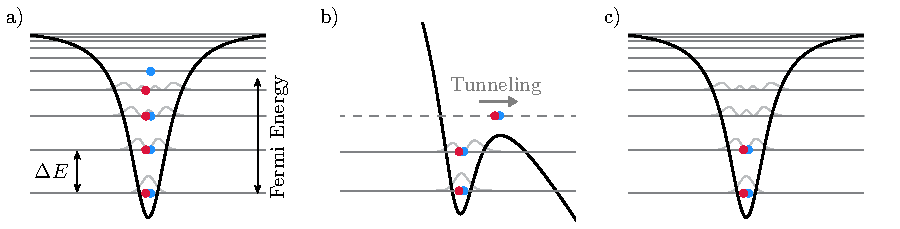
\includegraphics{fig-ai/preparation.pdf}
    \caption{
        \textbf{Deterministic preparation via spilling.}
        (a) Fermionic atoms are initially loaded into a tightly confined optical tweezer, forming a Fermi sea occupying the approximately 1D harmonic oscillator levels up to the Fermi energy. 
        (b) A magnetic field gradient tilts the potential, and the trap depth is lowered such that atoms above a defined spill level tunnel out. 
        (c) This procedure leaves a well-defined number of atoms in the lowest energy states, with a preparation fidelity of approximately 95\%. 
        Blue and red dots denote atoms in different spin states; gray curves indicate the bound-state wavefunctions.
    }
    \label{fig:preparation}
\end{figure}



\textbf{Tweezer loading.} We begin by preparing a spin-balanced mixture in the two lowest hyperfine states, $|1\rangle$ and $|2\rangle$, using a compressed magneto-optical trap (MOT). The atoms are initially loaded into a crossed ODT, where we perform evaporative cooling. This follows closely the sequence described in~\cite{culemann_construction_2024}.

After cooling, the atoms are transferred into a tightly focused optical tweezer potential. The loading process relies on the so-called \emph{dimple trick}~\cite{zurn_few-fermion_2012}, where a tightly confined but deep tweezer potential is superimposed onto the wider ODT reservoir. Because the tweezer affects only a small region of the total cloud, the global temperature $T$ remains approximately unchanged, while the local chemical potential is enhanced. In this regime, the average occupation number $\bar{n}(E_i)$ of a single-particle state $i$ with energy $E_i$ follows the Fermi-Dirac distribution:
\begin{equation}
    \bar{n}(E_i) = \frac{1}{e^{(E_i - \mu)/k_B T} + 1}.
\end{equation}
If the energy gap between the ground state $E_0$ and the Fermi energy $E_F$ is increased such that $(E_0 - E_F) / k_B \gg T$, then $\bar{n}(E_0) \rightarrow 1$. This ensures near-unity occupation of the lowest level, which provides an ideal starting point for deterministic preparation. In our experiment, this condition is achieved by ramping on the tweezer adiabatically while continuing evaporation inside the tweezer. The full loading and cooling sequence is depicted in Fig.~\ref{fig:preparationseq}.

\textbf{Deterministic few-body preparation via spilling.} To isolate a well-defined number of atoms in the lowest motional states of the tweezer, we use the \emph{spilling technique}, as described in~\cite{zurn_few-fermion_2012, holten_pauli_2022}. This method relies on tilting the potential with a magnetic field gradient and reducing the trap depth to allow atoms above a threshold energy to tunnel out. 
The resulting states are shown in Fig.~\ref{fig:preparation}. \red{See Appendix for details.}
% The energy levels and wavefunctions of the effective 1D potential under combined optical and magnetic fields were obtained numerically using a finite-difference method and the Thomas algorithm.

The spilling sequence is performed at a magnetic field of 527\,G, where the two spin states are nearly non-interacting. A magnetic field gradient of 20\,G/cm creates a linear tilt, and the tweezer power is lowered to a value that sets the spill threshold. After a short tunneling time, the trap depth is ramped back up to recapture the remaining atoms. By empirically optimizing these parameters, we achieve deterministic preparation of two atoms per tweezer with a fidelity of approximately 95\,\%. This sequence results in high-fidelity preparation within a total experimental cycle time of less than 2\,s.

% Стоит сказать, что система достаточно симметрична по отношению к уменьшению tweezer depth во время spilling или увеличению градиента. 


\begin{figure}
    \centering
    \addletter{140}{a}
    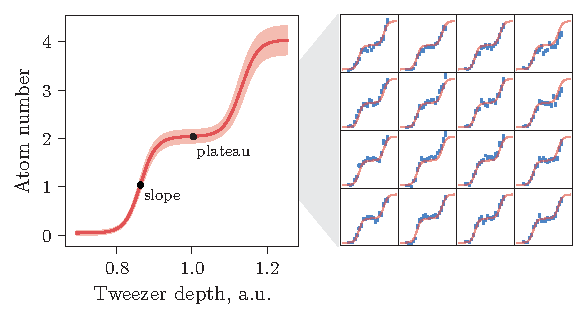
\includegraphics{fig-ai/step-plot-joined.pdf}
    \phantom{42}
    \addletter{140}{b}
    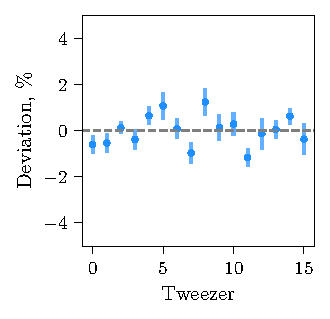
\includegraphics{fig-py/step-plot-balance.pdf} % 0.6 +- 0.2
    % 
    % 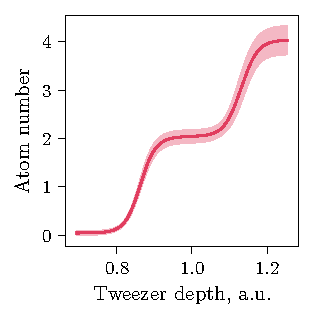
\includegraphics{fig-py/step-plot.pdf}
    % 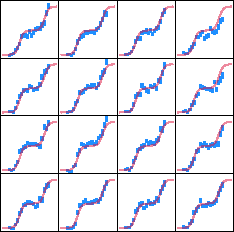
\includegraphics{fig-py/step-plot-inset.pdf}
    \caption{
        \textbf{Step plot.}
        (a) 
        Atom number as a function of tweezer depth during the spilling sequence. 
        % Plateaus correspond to quantized energy levels of the 1D harmonic oscillator. 
        Step plots for each tweezer in the $4 \times 4$ array are shown on the right. The average fit is shown as a solid red line, with standard deviation across sites indicated by the shaded area. 
        (b) Relative deviation of the fitted sigmoid centers for each tweezer after SVF balancing. The standard deviation is $0.7(2)\%$, which is well within the plateau width ($\pm 5\,\%$), ensuring sufficient uniformity for array-wide spilling. \red{$\chi^2$?}
        % All measurements were performed in this work using atom-based measurements and SVF-balanced tweezer depths.
    }
    \label{fig:stepplot}
\end{figure} % Loading, cooling, spilling in single tweezer

\subsection{Tweezer control} \label{subsec:control}
% !TEX root = ../master-thesis.tex

\textbf{Frequency to position mapping.}
To extract the local intensities $P_{ij}$ from camera images, we need to determine which pixels correspond to which tweezer sites. For this purpose, we define an affine transformation from the drive frequency space $(\omega_{\mathrm{hor}}, \omega_{\mathrm{ver}})$ to image plane coordinates $(x, y)$:
\begin{equation*}
    \vc{r} = H \vc{\omega},
    \hspace{5 mm} \Leftrightarrow \hspace{5 mm} 
    \begin{pmatrix}
        x \\ y
    \end{pmatrix} = \begin{pmatrix}
        h_{11} & h_{12} & h_{13} \\
        h_{21} & h_{22} & h_{23}
    \end{pmatrix} 
    \begin{pmatrix}
        \sub{\omega}{hor} \\
        \sub{\omega}{ver} \\
        1
    \end{pmatrix}.
\end{equation*}
Here, $H$ is a $2 \times 3$ matrix calibrated from a set of measured spot positions. For example, one can measure $\vc{r}_j$ for random frequency vectors $\vc{\omega}_j \in [\omega_{\mathrm{min}},\, \omega_{\mathrm{max}}]$, construct the matrices $\omega_{ij}$ with $i \in \{\mathrm{hor}, \mathrm{ver}\}$ and $r_{ij}$ with $i \in \{x, y\}$, and solve the least-squares problem:
\begin{equation}
    r = H \omega,
    \hspace{0.5cm} \Rightarrow \hspace{0.5cm}
    r \omega^\mathrm{T} = H \omega \omega^\mathrm{T}
    \hspace{0.5cm} \Rightarrow \hspace{0.5cm}
    r \omega^\mathrm{T} \left(\omega \omega^\mathrm{T}\right)^{-1} = H.
    \label{eq:linreg-freq2pos}
\end{equation}

This transformation defines a region of interest around each tweezer, within which we compute the integrated pixel intensity after background subtraction. The resulting values are proportional to the optical powers $P_{ij}$.

\textbf{Linear reconstruction.}
The mapping from input amplitudes $\vc{a}$ to optical power is approximated by Eq.~\eqref{eq:taylerexp}. In the regime $a_i \in [0.85, 0.95]$, a linear approximation is sufficient\footnote{
    For wider amplitude ranges, higher-order terms can be added to the model. However, this is unnecessary in the present context.
}. We construct the Jacobian matrix $F'_{ji}$ by fitting a linear regression model to a dataset of amplitude–intensity pairs. The resulting crosstalk matrix is shown in Fig.~\ref{fig:control}b. It is approximately diagonal, with comparable diagonal entries and off-diagonal elements typically reaching up to 30\% in magnitude relative to the diagonal, due to power redistribution between neighboring tones. Crosstalk between the horizontal and vertical AODs remains negligible.

The quality of the linear fit for the $4 \times 4$ array is illustrated in Fig.~\ref{fig:control}e. The total intensity (Fig.~\ref{fig:control}d) scales linearly with the average input amplitude, yielding $R^2 > 0.99$. Relative residuals are normally distributed with width $0.3\%$, confirming the applicability of the model in this range.

\textbf{Power-aware optimization.}
\grey{In the presence of limited laser power and finite AOM diffraction efficiency, we prefer solutions where all amplitudes remain close to 1. This preference can be incorporated into the optimization objective. In addition to minimizing intensity imbalance, we penalize deviations of the average amplitudes from a target value (e.g., 0.9).}



\begin{figure}
    \centering
    \addletter{170}{a}
    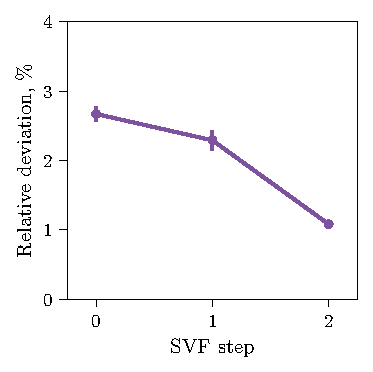
\includegraphics{fig-py/svf-avg.pdf}
    \addletter{170}{b}
    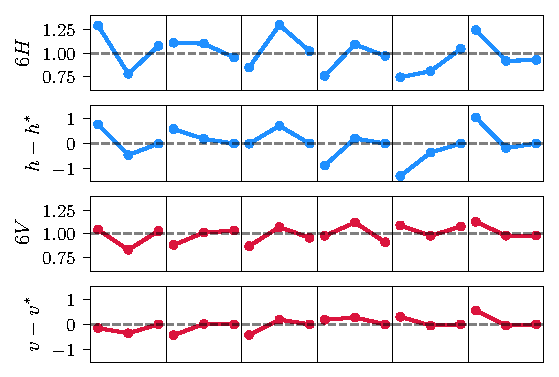
\includegraphics{fig-py/svf.pdf}
    \caption{
        \textbf{Single-value feedback (SVF) optimization for a $6 \times 6$ tweezer array.}
        (a) Relative deviation of effective powers $P_j$ across the array during successive SVF steps, quantified as $\mathrm{std}(P_j)/\langle P_j \rangle$. The initial point corresponds to camera-based balancing; subsequent iterations apply SVF with feedback rates $\gamma = 1/20$ and $\gamma = 1/40$. Further iterations did not yield statistically significant improvements. 
        (b) Retrieved horizontal powers $H_i$ and vertical powers $V_j$ (top and third rows), along with corresponding deviations of driving amplitudes from their final target values, $h - h^*$ and $v - v^*$. The recovered $H$, $V$ vectors are extracted from the photon count matrix $M_{ij}$ using factorization as described in \eqref{uv-decomposition}.
    }
    \label{fig:svf}
\end{figure}

\subsection{Tweezer depth balancing} \label{subsec:balancing}
% !TEX root = ../master-thesis.tex



\grey{It is also possible to calibrate each AOD independently, without relying on an SVD-based approach. This alternative was not tested in the scope of this work. However, it is worth emphasizing that the SVD-based method is guaranteed to work even for double-AOD configurations~[ref], where crosstalk between the two directions can be significantly stronger.}

Precise control over the depth of each optical tweezer is essential for preparing few-fermion systems via spilling techniques. In our setup, each tweezer is initially loaded with approximately \red{100} atoms, which are then selectively removed by ramping down the potential depth. The number of remaining atoms as a function of spill power $x_{\mathrm{sp}}$ exhibits a quantized staircase structure, reflecting the discrete energy levels of the 1D harmonic oscillator. This behavior can be characterized by a step plot~\cite{holten_pauli_2022}.

\textbf{Step plot.}
To characterize this behavior in our tweezer array, we measure step plots for all sites simultaneously. Figure~\ref{fig:stepplot}a shows the result for a $4 \times 4$ array. For each value of $x_{\mathrm{sp}}$, we acquire 70 experimental realizations and compute the average photon signal per site. 
% This signal serves as a robust proxy for atom number. In contrast to single-atom counting, this approach is parameter-free and effective even for large initial occupancies.

\textbf{Uniformity characterization.}
To quantify depth inhomogeneity across the array, we fit each step trace with a sigmoid function:
\begin{equation*}
    \sigmoid(x) = \frac{A_j}{1 + \exp\left(-(x - x_j)/\sigma_j\right)},
\end{equation*}
where $x_j$ denotes the center of the step and $\sigma_j$ its width for tweezer $j$. We define a relative uniformity metric as $\std(x_j) / \langle x_j \rangle$. After camera-based balancing (Sec.~\ref{subsec:control}), this metric typically yields $\sim 3\%$, which is insufficient for deterministic preparation across the array. A more precise balancing procedure is therefore required.




\textbf{Single-value feedback.}
To further improve uniformity, we apply an iterative atom-based feedback scheme. Rather than fitting full step plots, we operate at a single point on the slope of the transition, near the half-filling level $A_j / 2$. At this point, the sigmoid can be approximated by a linear response:
\begin{equation*}
    \sigmoid(x) \approx \frac{A_j}{4 \sigma_j} x - \frac{A_j x_j}{4 \sigma_j},
\end{equation*}
assuming $x_j \gg \sigma_j$.  In the feedback loop, we do not use the fitted sigmoid parameters directly. Instead, we measure a single photon-count matrix $M_{ij}$ and treat it as a linear proxy for the power matrix $P_{ij}$. Since the sigmoid offset $\mathrm{shift} = A_j x_j / (4 \sigma_j)$ is known from the fits, we approximate:
\begin{equation}
    \label{mp-propto}
    M_{ij} + \mathrm{shift} \propto P_{ij} = \Lambda H_i V_j.
\end{equation}
We then factorize this matrix using the method introduced in \eqref{uv-decomposition} and update the amplitudes according to:
\begin{equation*}
    h \rightarrow h + \gamma (H - H_0), \qquad
    v \rightarrow v + \gamma (V - V_0),
\end{equation*}
where $(H_0, V_0)$ is the target point, and $\gamma$ is the feedback rate. This model-free procedure avoids full sigmoid fitting and operates directly on experimental measurements.

Figure~\ref{fig:stepplot}b shows the result of applying this single-value feedback (SVF) protocol to a $4 \times 4$ array. After five iterations, the relative deviation of the fitted step centers is reduced to $0.7(2)\%$, well within the plateau width (typically $\pm5\%$), enabling deterministic state preparation across the full array. \red{Add fig. with single value feedback progress.}

Figure~\ref{fig:svf}a shows the process of applying the SVF protocol to a $6 \times 6$ array. The proportionality coefficient in \eqref{mp-propto} is $A/4\sigma \sim 10(1)$ (the average value is chosen for the plot) for our experiment.

\subsection{Tweezer movement} \label{subsec:tweezer-movement}
% !TEX root = ../master-thesis.tex

% tweezer_movement.tex

% \subsection{Tweezer movement} \label{subsec:tweezer-movement}




% \textbf{Tweezer movement}.
In experiments aiming at deterministic preparation and site-resolved imaging of individual ultracold atoms, precise and robust control over tweezer positions is crucial. In the present setup, while the Matter-Wave Magnifier (MWM) remains under development, single-atom imaging is achieved by initially positioning optical tweezers sufficiently far apart to individually resolve atoms. Specifically, atoms are loaded from the optical dipole trap (ODT) into tweezer potentials at an initial separation of $5\mu$m. Subsequently, this spacing is gradually increased to approximately $50\mu$m by smoothly varying the driving frequencies of the acousto-optic deflectors (AODs), enabling direct optical resolution without additional magnification.

% \textbf{Transport trajectory optimization.}
The protocol chosen for tweezer translation critically influences the fidelity of atom transport. Naively, atoms can be moved by linearly ramping tweezer frequencies; however, such linear trajectories often lead to significant atom loss due to non-adiabatic excitations induced by abrupt changes in acceleration. To mitigate these losses, a smoother trajectory known as the Minimum-Jerk Trajectory (MJT) is employed. This trajectory is derived by minimizing the functional associated with the time-integrated square of the third derivative of the position, known as the jerk $j(t) = \dddot{x}(t)$:
\begin{equation}
\mathcal{J}[x(t)] = \int_{0}^{T} \left(\frac{d^3 x(t)}{dt^3}\right)^2 dt,
\label{eq:mjt-functional}
\end{equation}
where $x(t)$ denotes the position and $T$ the total transport duration. Minimization of Eq.~\eqref{eq:mjt-functional}, subject to the boundary conditions of initial and final positions $x(0) = x_i$, $x(T) = x_f$, and zero initial and final velocities and accelerations, yields a polynomial form:
\begin{equation}
x(t) = x_i + (x_f - x_i)\left[10\left(\frac{t}{T}\right)^3 - 15\left(\frac{t}{T}\right)^4 + 6\left(\frac{t}{T}\right)^5\right].
\label{eq:mjt-solution}
\end{equation}
This smooth polynomial interpolation minimizes abrupt changes in acceleration, thereby reducing non-adiabatic excitation and atom loss during transport.

\begin{figure}
\centering
\addletter{85}{a}
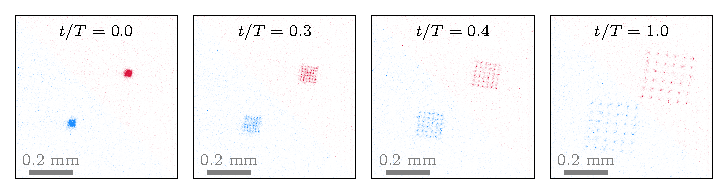
\includegraphics{fig-py/movement-inset.pdf} \\
\addletter{115}{b}
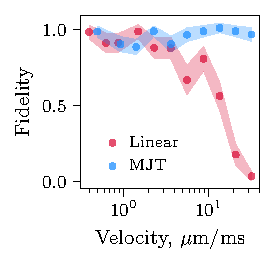
\includegraphics{fig-py/movement-1.pdf}
\hspace{1cm}
\addletter{115}{c}
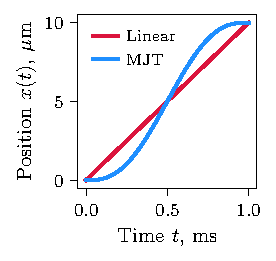
\includegraphics{fig-py/movement-2.pdf}
\caption[Characterization of tweezer transport protocols]{
\textbf{Characterization of tweezer transport protocols.}
(a) Snapshots at different fractions of the total transport duration, illustrating atom movement between initial and target tweezer positions during a typical experimental run.
(b) Comparison of transport fidelity as a function of velocity for the Minimum-Jerk Trajectory (MJT) and linear trajectory. Fidelity is defined as the probability of detecting an atom after transport, conditional on its initial presence.
(c) Position versus time curves for MJT and linear transport trajectories.
Data points correspond to measurements, shaded areas represent standard deviation across realizations.
}
\label{fig:movement}
\end{figure}


% \textbf{Experimental characterization of trajectories.}
To experimentally validate the efficacy of MJT compared to linear transport, systematic measurements were conducted. The fidelity of transport is defined as the probability of detecting an atom after transport, conditional upon its initial presence. As depicted in Fig.~\ref{fig:movement}b, the MJT significantly outperforms the linear trajectory across a broad range of transport velocities. These measurements are obtained by initially holding atoms stationary for a fixed duration, thereby establishing a baseline population expected without transport-induced losses. Subsequently, atoms are transported along a zigzag path (forward and backward), and transport fidelity is measured relative to this baseline. Given the relatively low mass of $^6$Li atoms, high transport velocities are achievable. Indeed, at typical experimental transport velocities of approximately $10\mu$m/ms, MJT achieves fidelities exceeding 99\%, as demonstrated in Fig.~\ref{fig:movement}b. This highlights MJT as the trajectory of choice for efficient and robust tweezer movement.

% \textbf{Trajectory profiles and experimental snapshots.}
Detailed position versus time curves for both linear and MJT trajectories are shown in Fig.\ref{fig:movement}c. The MJT profile distinctly smooths acceleration and deceleration phases compared to the linear ramp, clearly illustrating the reduction in jerk. Correspondingly, experimental snapshots at various fractions of the total transport duration, depicted in Fig.\ref{fig:movement}a, visually confirm smooth and uniform atomic redistribution between initial and final positions. Each snapshot represents fluorescence images averaged over ten experimental realizations, confirming reproducible atom transport without significant losses or heating.

In summary, the implementation and systematic characterization of MJT for tweezer translation provides a critical improvement in transport fidelity compared to simple linear movements. The derived and experimentally validated MJT ensures minimal atom loss, thereby facilitating precise atom arrangement. 



\subsection{Tweezer loading} \label{subsec:tweezer-loading}
% !TEX root = ../master-thesis.tex

% tweezer_loading.tex
% \subsection{x Tweezer loading} \label{subsec:tweezer-loading}



% \textbf{Tweezer loading}.
Even with meticulous balancing of tweezer intensities, residual imperfections inevitably persist in the final atom distributions. These imperfections arise from several distinct contributions, including tweezer movements, loading processes from the optical dipole trap (ODT), and fluorescence imaging. The present subsection specifically examines the influence of loading atoms from the ODT into the tweezer array, isolating this particular contribution from other experimental stages.

% \textbf{Characterization of atom loading from the ODT.}
To systematically investigate loading effects, atom numbers in individual tweezers are measured directly after the \red{pre-evaporation} stage and prior to spilling. At this intermediate stage, the number of atoms per tweezer is inferred from the fluorescence signals recorded by the nuvu camera. Combining previously obtained calibration data from step plots and single-atom counting experiments (Sec.~\ref{sec:imaging}), approximately 30 photons per atom are expected to be detected by the camera, allowing quantitative estimation of atom populations per tweezer.

% \textbf{Constraints on minimal inter-tweezer spacing.}
In the current setup, the minimum feasible spacing between tweezers is restricted to approximately $5,\mu$m. Attempts to further reduce this separation consistently resulted in elevated atom losses, presumably due to parametric heating effects associated with closely spaced potentials. Although stroboscopic methods—rapidly alternating between different AOD configurations—might mitigate these heating effects, such approaches require further systematic investigation and remain topics for future research. A dedicated characterization of minimal achievable spacing and associated atom retention rates is necessary and will be addressed in forthcoming studies \red{(add plot on the minimum distance between atoms in future)}.

% \textbf{Dragging approach for enhanced loading.}
A preliminary investigation explored an alternative strategy: the dragging method, in which an array of tweezers is adiabatically translated through the ODT during loading. This approach allowed loading of larger tweezer arrays compared to the stationary loading method. However, despite its promise, the dragging method exhibited potential heating issues both in the ODT reservoir and within the tweezers themselves. The effectiveness of dragging critically depends on an accurate balance between tweezer and ODT depths, and careful optimization of these parameters also remains a necessary direction for future research.

% \textbf{Observed inhomogeneity in tweezer loading.}
With stationary loading at a fixed $5,\mu$m spacing, systematic spatial inhomogeneities are consistently observed, particularly affecting the corner regions of the tweezer array. This effect is illustrated clearly in Fig.\ref{fig:loading-from-odt}a, which shows an averaged atom distribution for a $6\times6$ tweezer array directly after loading from the ODT. Atom occupancy at corner sites is markedly reduced relative to central sites. A quantitative assessment of loading imbalance is provided in Fig.\ref{fig:loading-from-odt}b, depicting the measured atom number distribution for a uniformly powered $4\times4$ tweezer array. The corners show systematically lower populations compared to central positions.

% \textbf{Improvement via manual intensity adjustments.}
To overcome this intrinsic loading imbalance, a manual redistribution of tweezer intensities was performed using the previously measured camera-based crosstalk matrix. Specifically, the intensities of corner tweezers were deliberately increased relative to central tweezers to compensate for the lower initial loading rates. This simple yet effective manual intervention improved corner loading significantly, increasing atom numbers at corner positions by approximately 20\% as demonstrated in Fig.~\ref{fig:loading-from-odt}c. Consequently, this intensity adjustment facilitated more homogeneous atom distribution and higher fidelity in subsequent state preparation procedures.

In summary, careful analysis and targeted intensity adjustments during the ODT loading phase substantially reduce residual inhomogeneities in atom occupancy. However, further improvements and more systematic methods—including minimal spacing optimization, stroboscopic techniques, and dragging approaches—represent valuable areas for continued research.


\begin{figure}
    \centering
    \addletter{90}{a}
    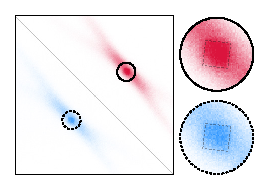
\includegraphics{fig-ai/loading-from-odt-1-ai.pdf}
    \phantom{42}
    \addletter{90}{b}
    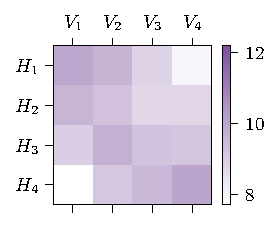
\includegraphics{fig-py/loading-from-odt-2.pdf}
    \phantom{42}
    \addletter{90}{c}
    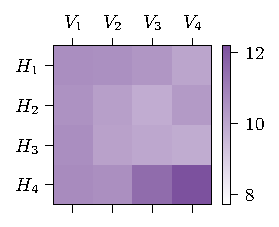
\includegraphics{fig-py/loading-from-odt-3.pdf}
    \caption{
    \textbf{Inhomogeneous loading from ODT to tweezer arrays.}
    (a) Atom distribution for a $6\times6$ array (averaged over 10 realizations), demonstrating inhomogeneous loading from the optical dipole trap (ODT).
    (b) Observed atom number distribution for a uniformly powered $4\times4$ tweezer array, revealing systematically lower loading efficiency at corners (averaged over 30 realizations).
    (c) Improved uniformity after manual adjustment of tweezer intensities, specifically enhancing corner powers (averaged over 30 realizations).
    }
    \label{fig:loading-from-odt}
\end{figure}

\subsection{Spin-selective spilling} \label{subsec:spin-selective-spilling}
After balancing the tweezer depths and performing standard spilling to prepare unit filling (one atom in state $\ket{1}$ and one in $\ket{2}$ per site), atoms in a selected spin state can be selectively removed while leaving the other unaffected. This enables the preparation of arbitrary spin-resolved configurations, a crucial ingredient for bottom-up simulation of spinful many-body systems.

\textbf{Magnetic-field dependence.}
The key idea relies on the difference in magnetic moments between the hyperfine ground states. As shown in Fig.~\ref{fig:li6levels}b, the energy of state $\ket{2}$ exhibits a maximum near $27\,\mathrm{G}$, where its magnetic moment vanishes: $\mu_{|2\rangle} = \partial E / \partial B = 0$. In contrast, state $\ket{1}$ has a sizable negative magnetic moment at this field \red{(write down value)}. As a result, when a magnetic field gradient is applied at $B = 27\,\mathrm{G}$, only atoms in state $\ket{1}$ experience a significant force and are spilled from the traps.

\textbf{Spin-selective removal.}
The experiment starts with a $\ket{1}$–$\ket{2}$ spin mixture at unit filling in each tweezer. The magnetic field is ramped to $27\,\mathrm{G}$, and a field gradient is applied. This results in spin-selective spilling: atoms in state $\ket{1}$ are removed, while those in $\ket{2}$ remain confined.

The crossed AOD configuration enables control over the local optical power $P_{ij}$ through factorized amplitudes, such that $P_{ij} = H_i V_j$. This allows us to define arbitrary rank-1 intensity masks and thus selectively apply spilling to specific subsets of sites. 
% In this way, we can prepare structured spin patterns such as stripes, checkerboards, or arbitrary factorized configurations.

This protocol enables single-shot removal of state $\ket{1}$ atoms without perturbing state $\ket{2}$, providing a flexible method for initializing spin-imbalanced or spatially patterned states. The performance of the method in terms of selectivity and overall fidelity is summarized in \red{Fig.~?}. Sequential applications of such steps to prepare arbitrary configurations are discussed in Sec.~\ref{subsec:arbitrary-occupation-loading}.


\subsection{Arbitrary occupation loading} \label{subsec:arbitrary-occupation-loading}
% !TEX root = ../master-thesis.tex

The ability to prepare arbitrary atom configurations is a key ingredient for bottom-up quantum simulation. After obtaining unit filling for both spin states (as discussed in Sec.~\ref{subsec:balancing} and \ref{subsec:spin-selective-spilling}), we implement a multi-stage spilling sequence that enables spin- and site-resolved initialization of arbitrary patterns.

The loading sequence proceeds in several steps:
\begin{enumerate*}
    \item Prepare a $\ket{1}$–$\ket{2}$ spin mixture with unit filling across the tweezer array.
    \item Perform global spilling steps to remove atoms from factorized intensity patterns $P_{ij}$, affecting both spin states.
    \item Apply spin-selective spilling steps to remove atoms in state $\ket{1}$ from additional factorized subsets of sites.
    \item Flip the remaining atoms $\ket{1} \leftrightarrow \ket{2}$ using a microwave $\pi$-pulse.
    \item Repeat spin-selective spilling to further refine the configuration
\end{enumerate*}

\textbf{Factorized removal.}
Each spilling step removes atoms from sites where the local tweezer depth $P_{ij}$ falls below a certain threshold. Since we can impose any rank-1 intensity mask $P_{ij} = H_i V_j$, it is possible to tailor the removal region to arbitrary product forms. To remove a single atom at site $(i', j')$, for example, we reduce $H_{i'}$ and $V_{j'}$ by a factor $\eta < 1$ and simultaneously increase the global power by $\eta$. This yields a relative intensity of $1/\eta$ at the intersection, while leaving all other sites unchanged or increased in depth. In this way, we can reliably isolate and remove atoms from any desired factorized subset.

\textbf{Boolean decomposition.}
We represent the cumulative removal pattern as a binary matrix $W_{ij}$, where $W_{ij} = 1$ indicates that the atom at site $(i, j)$ has been removed. Each spilling operation adds a binary outer product $u^\lambda_i v^\lambda_j$ via Boolean logic ($1 + 1 = 1$). An arbitrary target pattern can therefore be reached through a sequence of such operations:
\begin{equation}
    \label{eq:ebmf}
    W_{ij} = \bigvee_{\lambda=1}^{r} u^\lambda_i v^\lambda_j,
\end{equation}
which defines the exact Boolean matrix factorization (EBMF) of the removal matrix. In the worst case, any binary $n \times n$ matrix admits such a decomposition using at most $n$ steps.

\textbf{Optimal EBMF.}
While a naive strategy—such as row- or column-wise removal—may require up to $n$ iterations, we find that optimal EBMF often reduces this number. The problem of finding an exact Boolean matrix factorization with minimal rank is known to be NP-complete~\cite{orlin_contentment_1977} and NP-hard to approximate~\cite{gruber_inapproximability_2007}. Nevertheless, for arrays up to $10 \times 10$, optimal decompositions can be computed in a few seconds using a SAT solver. These improvements are particularly useful for minimizing experimental cycle time and improving overall sequence fidelity. A full discussion of the EBMF algorithm and its implementation is presented in Appendix.




\newpage
% --------------------------------------------------------------------------------------
\section{Fermi-Hubbard model: numerical approaches and simulations} \label{sec:fhmodel}
% --------------------------------------------------------------------------------------

\subsection{Introduction}
% !TEX root = ../master-thesis.tex

% --------------------------------------------------------------------------------------
% Intro
% --------------------------------------------------------------------------------------

% \textbf{Overview.}
Understanding the dynamics of isolated quantum systems remains one of the central goals of contemporary many-body physics. Over the last decades, considerable progress has been made in classifying and probing different dynamical regimes, from thermalizing phases consistent with conventional statistical mechanics to exotic non-ergodic phases that violate the Eigenstate Thermalization Hypothesis (ETH). Among these, the Fermi-Hubbard model has emerged as a paradigmatic platform for studying the interplay of interactions, quantum statistics, and disorder in strongly correlated systems.

In the clean, disorder-free limit, the Fermi-Hubbard model exhibits rich equilibrium physics, including Mott insulators, spin ordering, and pseudogap phenomena relevant to high-temperature superconductivity \cite{esslinger_fermi-hubbard_2010}. However, the model also serves as a fertile ground for exploring nonequilibrium phenomena, such as quantum quenches, relaxation, transport, and entanglement dynamics — especially when generalized to include disorder or spatial inhomogeneities.

Recently, theoretical and experimental attention has increasingly shifted toward the role of disorder in quantum many-body dynamics. It is now understood that disorder can lead to fundamentally different behaviors depending on the presence or absence of interactions. For instance:
\begin{itemize}
	\item In the absence of interactions, disorder induces \textit{Anderson localization}, which prevents particle diffusion and leads to persistent memory of initial conditions \cite{anderson_absence_1958}.
	\item When interactions are present, the system may enter the regime of \textit{many-body localization (MBL)}, characterized by the absence of thermalization and slow unbounded entanglement growth \cite{basko_metalinsulator_2006,nandkishore_many-body_2015}.
	% , and emergent local integrals of motion
	\item In contrast, when disorder is weak or absent, the system typically evolves toward local thermal equilibrium, consistent with the predictions of \textit{ETH} \cite{deutsch_quantum_1991,srednicki_chaos_1994}. 
\end{itemize}

These dynamical phases (\emph{thermal, Anderson-localized, and MBL}) are typically distinguished through the behavior of local observables, spectral statistics, and the dynamics of quantum correlations. Their interplay is especially rich in two dimensions, where the presence of more complex geometry, potential mobility edges, and rare-region effects make the dynamical phase diagram both challenging and intriguing.

From an experimental standpoint, studying such phenomena requires precise control over initial states, evolution Hamiltonians, and high-fidelity measurements of observables at the single-site level. This thesis presents a platform that provides such control, combining deterministic initialization of fermionic states in a two-dimensional tweezer array with programmable evolution under the Fermi-Hubbard Hamiltonian and spin- and site-resolved imaging.

Compared to conventional optical lattice experiments, the tweezer-based approach offers several key advantages for nonequilibrium quantum simulation:
\begin{enumerate}
	\item \textit{Deterministic and programmable state preparation.} Using a sequence of global and spin-selective spilling operations, arbitrary configurations of fermionic atoms can be prepared with high fidelity. This capability enables initialization of tailored many-body states for probing specific dynamical scenarios, such as local quenches, domain-wall melting, or imbalance relaxation.
	\item \textit{Fast experimental cycle and large statistics.} The entire experimental sequence, including preparation, evolution, and measurement, completes in under two seconds, allowing up to $10^5$ experimental repetitions per day. This rapid repetition rate is crucial for averaging over disorder realizations and collecting sufficient statistics for dynamical observables.
	\item \textit{Spin- and site-resolved detection.} The developed imaging system supports fluorescence-based, single-shot discrimination of atomic spin states on individual lattice sites. This enables direct access to observables such as density profiles $\langle n_j \rangle$, magnetization $\langle \sigma^z_j \rangle$, and spin correlations $\langle \sigma^z_i \sigma^z_j \rangle$ — all of which are sensitive to the system's dynamical regime.
\end{enumerate}

In tandem with experimental capabilities, in this work a numerical simulation package was developed for modeling real-time dynamics in finite-size Hubbard systems. The package combines exact diagonalization (ED) for small systems and Krylov subspace methods for larger Hilbert spaces (up to $10^9$ dimensions), and supports evaluation of observables and entanglement entropy in arbitrary geometries and disorder realizations.

Together, these tools enable a systematic exploration of the dynamical phase diagram of the disordered Fermi-Hubbard model in two dimensions. By leveraging control over initial conditions, disorder strength, and interactions, as well as the ability to access key observables, one can address central questions in nonequilibrium many-body physics: What determines whether a system thermalizes? When does localization persist in the presence of interactions? How do correlations and entanglement spread in different regimes?

In the following subsections, we review the theoretical framework underpinning these questions, beginning with the concept of thermalization in isolated quantum systems.

 % What we want to simulate and why

\subsection{Dynamical phases}
% !TEX root = ../master-thesis.tex


% --------------------------------------------------------------------------------------
% Thermalization
% --------------------------------------------------------------------------------------


\textbf{Thermalization}.
A fundamental question in quantum many-body physics concerns how and under which conditions an isolated quantum system approaches thermal equilibrium. Intuitively, thermalization implies that after sufficient evolution time, local observables lose memory of the system's initial conditions and approach steady-state values corresponding to thermodynamic equilibrium \cite{khlebnikov_thermalization_2014}. To formalize this concept, consider an isolated quantum system described by a Hamiltonian $\hat{H}$, evolving from an initial state $\ket{\psi_0}$, which can be expanded in the eigenbasis ${\ket{E_j}}$ of the Hamiltonian with eigenenergies $\varepsilon_j$ as follows:
\begin{equation*}
\ket{\psi(t)} = \sum_{j=1}^{\mathcal{N}} c_j e^{- i \varepsilon_j t} \ket{E_j},
\label{eq:evolution}
\end{equation*}
where the coefficients are $c_j = \bk{E_j}{\psi_0}$, and $\mathcal{N} = \dim\mathcal{H}$ is the dimension of the Hilbert space.

For an arbitrary observable $\hat{A}$, its expectation value at time $t$ is given by:
\begin{equation*}
A(t) = \bk{\psi(t)}[\hat{A}]{\psi(t)}
= \sum_{j,k} \bar{c}k c_j e^{-i (\varepsilon_j - \varepsilon_k) t} \bk{E_k}[\hat{A}]{E_j}.
\label{eq:observable_time}
\end{equation*}
Expanding this further, one separates diagonal and off-diagonal contributions:
\begin{equation}
A(t) = \sum_j |c_j|^2 \bk{E_j}[\hat{A}]{E_j}
+ \sum_{k \neq j} c_j \bar{c}_k e^{-i (\varepsilon_j - \varepsilon_k) t} \bk{E_k}[\hat{A}]{E_j}.
\label{eq:At_expanded}
\end{equation}

Thermalization at large times, $t \gg \tth$, implies that the observable reaches a steady-state value $A(E)$ with small fluctuations around this average, where $E = \bk{\psi_0}[\hat{H}]{\psi_0}$ is the initial energy of the system:
\begin{equation*}
A(t \gg \tth) = A(E) + \text{small fluctuations}.
\label{eq:thermal_limit}
\end{equation*}

Analyzing Eq.~\eqref{eq:At_expanded}, the condition for small fluctuations around a steady-state value requires the off-diagonal matrix elements $\bk{E_k}[\hat{A}]{E_j}$, $k\neq j$, to be sufficiently small. Indeed, due to the large number of off-diagonal terms ($\sim \mathcal{N}^2$), their contributions could, in principle, sum up to large fluctuations. To suppress such fluctuations, one typically assumes these off-diagonal matrix elements to be negligible or effectively random, scaling as $1/\sqrt{\mathcal{N}}$.

Furthermore, to ensure that the steady-state expectation value $A(E)$ does not depend sensitively on initial conditions, one additional criterion is necessary: the diagonal elements $\bk{E_j}[\hat{A}]{E_j}$ must vary smoothly with energy:
\begin{equation*}
\bk{E_j}[\hat{A}]{E_j} \approx A(\varepsilon_j),
\end{equation*}
where $A(\varepsilon)$ is a continuous and smooth function of energy $\varepsilon$. Under these assumptions, if the initial state $\ket{\psi_0}$ occupies energy eigenstates within a sufficiently narrow energy window $\Delta E$, such that the variation $\partial_E A(E)\Delta E$ is small, we can approximate:
\begin{equation*}
A(t \gg \tth) \approx \sum_j |c_j|^2 A(\varepsilon_j) \approx A(E).
\end{equation*}

The conditions described above constitute the Eigenstate Thermalization Hypothesis (ETH), first introduced by Deutsch \cite{deutsch_quantum_1991} and later developed by Srednicki \cite{srednicki_chaos_1994}. ETH thus posits that individual eigenstates of chaotic quantum many-body systems already encode thermal equilibrium properties, and as long as the system's initial state overlaps with sufficiently many such eigenstates within a narrow energy band, observables will dynamically thermalize at large times.

It is important to note that for isolated quantum systems, the global state remains pure at all times, as indicated by the purity condition $\tr(\rho^2) = 1$. In contrast, a genuinely thermal mixed state would exhibit $\tr(\rho^2) < 1$. Thus, the concept of thermalization in isolated quantum systems pertains specifically to observables rather than the full density matrix. This subtlety motivates the interest in subsystem dynamics: if the total system is partitioned into subsystems $\Omega_1$ and $\Omega_2$, the reduced density matrix $\rho_1 = \tr_{\Omega_2} \rho$ might indeed become thermal (mixed), while subsystem $\Omega_2$ serves effectively as a thermal bath. This scenario represents a broader context beyond the current discussion but remains an intriguing direction for future experimental and theoretical exploration.

Finally, one should acknowledge the possibility of observable-dependent thermalization. Given the ETH criteria, it is plausible that in certain quantum systems, some observables $\hat{A}_1$ might thermalize effectively, while others, $\hat{A}_2$, may not. Thus, thermalization is not universal, but rather depends on the observable and the particular properties of the quantum system under consideration.

To summarize, thermalization in isolated quantum systems, as described by ETH, occurs when local observables evolve towards stationary, thermal equilibrium values at long times, provided the system's eigenstates satisfy specific criteria regarding their energy dependence and off-diagonal matrix elements.

% --------------------------------------------------------------------------------------
% Anderson localization
% --------------------------------------------------------------------------------------

\textbf{Anderson localization}.
Localization phenomena in quantum systems provide striking examples of the breakdown of thermalization and transport, even in the absence of interactions. A fundamental example is Anderson localization, first theoretically described by P. W. Anderson in the seminal work \cite{anderson_absence_1958}, originally in the context of non-interacting electrons in disordered lattices. Anderson localization describes the scenario where the presence of disorder in the potential landscape leads to exponential localization of single-particle wavefunctions and consequently prevents diffusion.

Consider the single-particle Hamiltonian describing hopping of a particle on a lattice with nearest-neighbor tunneling amplitude $t$ and site-dependent random potentials $V_i$:
\begin{equation*}
\hat{H} = -t \sum_{\langle i,j\rangle} (c_i^\dagger c_j + c_j^\dagger c_i) + \sum_{i} V_i n_i,
\label{eq:anderson_ham}
\end{equation*}
where $c_i^\dagger$ and $c_i$ are fermionic creation and annihilation operators on lattice site $i$, and $n_i = c_i^\dagger c_i$ is the number operator. The potentials $V_i$ are typically taken from a random distribution, such as uniformly distributed $V_i \in [-W, W]$, where $W$ characterizes the strength of the disorder.

Anderson demonstrated that in one and two dimensions, any finite amount of disorder is sufficient to localize all eigenstates, rendering them exponentially localized around particular lattice sites. In three-dimensional systems, there exists a critical value of disorder strength, beyond which the system transitions from a metallic (extended) to an insulating (localized) phase \cite{abrahams_50_2010}.

The key consequence of Anderson localization is the absence of diffusion, reflected by the suppression of transport properties and conductivity. A particle initially localized around a particular lattice site remains effectively trapped in a finite spatial region for all times. The wavefunction amplitudes at distant sites decay exponentially:
\begin{equation*}
|\psi_j| \sim e^{-|j-j_0|/\xi},
\end{equation*}
where $\xi$ is known as the localization length, and $j_0$ is the localization center. Importantly, $\xi$ decreases with increasing disorder strength.

From the perspective of quantum dynamics and thermalization, Anderson-localized systems exhibit fundamentally different behavior compared to systems obeying the Eigenstate Thermalization Hypothesis (ETH). Specifically, observables in Anderson-localized systems typically retain memory of their initial conditions indefinitely, as the system cannot redistribute energy or particle number efficiently. Formally, the off-diagonal matrix elements of observables remain substantial and non-randomized, violating the conditions required by ETH for thermalization.

To illustrate this behavior, consider a single-particle observable, such as the local density at site $j$, $\hat{n}_j = c_j^\dagger c_j$. Starting from an initially localized wavefunction $\ket{\psi_0}$, the expectation value of the local density at site $j$ evolves as:
\begin{equation*}
n_j(t) = \bk{\psi(t)}[\hat{n}_j]{\psi(t)}.
\end{equation*}
For a fully Anderson-localized system, this quantity remains close to its initial value for sites near the initial localization center and does not relax toward a homogeneous distribution, contrasting sharply with the ETH scenario.

It is important to emphasize that Anderson localization relies crucially on the absence of interactions. The presence of even weak interactions between particles can significantly alter the localization properties, either destabilizing localization and restoring ergodicity (thermalization) or giving rise to more complex regimes such as many-body localization (MBL), which will be discussed in the next section.

Experimental investigations of Anderson localization have been successfully realized in various physical platforms, including ultracold atomic gases in disordered or quasiperiodic optical potentials \cite{billy_direct_2008, roati_anderson_2008}. These experiments confirm the theoretical predictions and demonstrate key signatures such as absence of transport and persistent spatial confinement.

Summarizing, Anderson localization represents a fundamental example of non-thermalizing quantum dynamics, where disorder-induced localization suppresses energy and particle transport. This phenomenon violates the Eigenstate Thermalization Hypothesis, leading to persistent memory effects and long-lived non-equilibrium states, providing a clear contrast to thermalizing quantum systems.


% --------------------------------------------------------------------------------------
% MBL
% --------------------------------------------------------------------------------------

\textbf{Many-body localization (MBL)}.
While Anderson localization establishes the absence of transport in non-interacting systems due to static disorder, the behavior of \emph{interacting} disordered systems remained an open question for decades. The key insight emerged from the realization that localization can persist even in the presence of interactions, giving rise to the phenomenon of many-body localization (MBL) \cite{basko_metalinsulator_2006,nandkishore_many-body_2015,abanin_colloquium_2019}. MBL represents a genuine breakdown of statistical mechanics in isolated quantum systems: despite having strong interactions and high energy density, such systems do not thermalize and retain long-time memory of their initial conditions.

The MBL regime is most naturally studied in the disordered Fermi-Hubbard model, where the Hamiltonian is:
\begin{equation*}
\hat{H} = -t \sum_{\langle i, j \rangle, \sigma} (c^\dagger_{i \sigma} c_{j \sigma} + \text{h.c.}) + U \sum_i n_{i \uparrow} n_{i \downarrow} + \sum_{i, \sigma} V_i n_{i \sigma}.
\label{eq:fh-mbl}
\end{equation*}
Here, $t$ is the tunneling amplitude, $U$ the on-site interaction strength, and $V_i$ the static disorder potential at site $i$. The presence of both interactions and disorder sets the stage for competition between delocalization (favored by tunneling and interactions) and localization (favored by disorder). Several observable features distinguish MBL from both Anderson localization and thermalization.

% \textbf{Key signatures of MBL.} 

\emph{Absence of thermalization.} Local observables retain memory of their initial values at arbitrarily long times. For example, if the system is initialized in a charge-density wave state, the imbalance between even and odd sites does not relax to zero:
\begin{equation*}
\mathcal{I}(t) = \frac{N_\text{even}(t) - N_\text{odd}(t)}{N_\text{even}(t) + N_\text{odd}(t)} \not\rightarrow 0 \quad \text{as} \quad t \to \infty.
\end{equation*}
Such behavior reflects the failure of the Eigenstate Thermalization Hypothesis (ETH).

\emph{Slow entanglement growth.} Despite the absence of thermalization, MBL systems can exhibit entanglement growth over time. A hallmark of the MBL phase is a \emph{logarithmic} increase of bipartite entanglement entropy:
\begin{equation*}
S(t) \sim \log t,
\end{equation*}
in contrast to linear growth in thermal phases and saturation in Anderson-localized systems. This growth is attributed to dephasing processes mediated by interactions \cite{nandkishore_many-body_2015,bardarson_unbounded_2012} and signals that MBL eigenstates are not strictly product states.

% \emph{Existence of local integrals of motion (LIOMs).} Theoretical studies suggest that the MBL phase is characterized by an extensive set of quasi-local conserved quantities — so-called LIOMs or $l$-bits — which commute with the Hamiltonian and are localized in space \cite{serbyn_local_2013,huse_phenomenology_2014}. These operators explain the persistence of memory and the suppression of transport.

% \emph{Poissonian spectral statistics.} Similar to Anderson-localized systems, MBL systems exhibit Poissonian level spacing distribution:
% \begin{equation}
% P(s) \sim e^{-s},
% \end{equation}
% where $s$ is the spacing between neighboring energy levels, normalized by the mean. This reflects the absence of level repulsion, indicating lack of quantum chaos. In contrast, thermalizing systems exhibit Wigner-Dyson statistics.

% \textbf{MBL vs. Anderson localization.}
Although both Anderson localization and MBL prevent transport and thermalization, their underlying mechanisms and dynamical signatures differ. Anderson localization arises purely from interference and is static. Entanglement entropy does not grow over time (beyond single-particle effects). MBL is an intrinsically interacting phenomenon. While transport is suppressed, interactions induce dephasing and allow for slow spreading of entanglement and correlations.

These differences manifest in observables such as site-resolved magnetization and entanglement entropy. For instance, in a system initialized with spin imbalance, Anderson localization preserves local magnetization indefinitely, while weak interactions in MBL lead to its decay — even though the system remains non-thermal in terms of density observables. Similarly, growth of subsystem entanglement entropy in MBL (but not in AL) allows clear dynamical distinction.



% characterized by: 

% vanishing of long-time imbalance in time evolution, 

% Crossing of spectral statistics: average $r$-value transitions from $\langle r \rangle \approx 0.39$ (Poisson) to $\langle r \rangle \approx 0.53$ (GOE) \cite{oganesyan_localization_2007}.

% Disappearance of entanglement plateaus and onset of volume-law scaling in eigenstates.


As disorder strength $W$ is decreased or interaction $U$ is increased, MBL eventually breaks down. Numerical studies identify a sharp transition between MBL and thermalizing phases. 
However, due to finite-size limitations, precise determination of the transition point remains challenging in two dimensions. Notably, stability of MBL in 2D and higher dimensions has been a subject of debate, with proposed “thermal avalanche” mechanisms \cite{de_roeck_stability_2017}. Nevertheless, recent experiments and numerics show robust signatures of MBL-like behavior in 2D systems on experimentally relevant timescales \cite{choi_exploring_2016,bordia_probing_2017,wahl_signatures_2019}.

% \textbf{Experimental relevance.} 
MBL has been observed in cold atom systems, trapped ions, and superconducting circuits. In particular, ultracold fermionic atoms in disordered optical lattices provide a clean platform for probing MBL \cite{schreiber_observation_2015,kondov_disorder-induced_2015,choi_exploring_2016}. Our experimental platform, offering spin- and site-resolved preparation and readout, is well-suited to systematically study MBL in 2D geometries — including its dynamics, spatial correlations, and response to engineered perturbations.

% \textbf{Summary.} MBL represents a fundamentally new dynamical phase of matter in which interactions and disorder combine to prevent thermalization. It differs from Anderson localization by exhibiting slow entanglement growth and a rich structure of quasi-local conservation laws. As such, MBL serves as a bridge between quantum statistical mechanics, information dynamics, and condensed matter physics.


% --------------------------------------------------------------------------------------
% Integrable limit
% --------------------------------------------------------------------------------------


\textbf{Integrable limit}.
An important baseline for understanding quantum thermalization and localization is the behavior of clean, non-interacting systems. In the absence of both interactions and disorder, many-body systems may become integrable — that is, they possess an extensive set of conserved quantities that constrain the dynamics. These systems do not thermalize \cite{abanin_colloquium_2019} in the conventional sense, as their dynamics remains quasi-periodic and retains detailed memory of the initial state. This regime provides a sharp contrast to both ETH-obeying thermal systems and disorder-induced localized phases.

Consider the Fermi-Hubbard model with $U = 0$ and $V_i = 0$, i.e., a system of non-interacting fermions hopping on a regular lattice:
\begin{equation*}
\hat{H}_0 = -t \sum_{\langle i,j \rangle, \sigma} \left( c_{i\sigma}^\dagger c_{j\sigma} + \text{h.c.} \right).
\label{eq:free_ham}
\end{equation*}
This model is diagonalizable in momentum space. The occupation number operators in the single-particle eigenbasis, $\hat{n}_k = c_k^\dagger c_k$, commute with the Hamiltonian and with each other, making them integrals of motion. Consequently, the time evolution of any observable is constrained by the conservation of mode occupations:
\begin{equation*}
\frac{d}{dt} \hat{n}_k(t) = 0 \quad \text{for all } k.
\end{equation*}

Such a structure leads to \textit{non-ergodic dynamics}: the system does not explore the full Hilbert space compatible with energy conservation. Instead, its evolution is confined to a restricted subspace determined by the initial conditions. As a result, local observables generally exhibit persistent oscillations or approach non-thermal steady states.

A common illustration is the expansion of a domain-wall initial state, where all fermions are localized on one half of the lattice. In a thermalizing system, this state would relax toward a uniform density. In the integrable limit, however, the density profile exhibits long-lived coherent oscillations, reflecting ballistic propagation of non-interacting wave packets.

% \textbf{Generalized Gibbs ensemble (GGE).}
% Since conventional thermal ensembles fail to describe long-time observables in integrable systems, a different statistical description is required. The appropriate object is the Generalized Gibbs Ensemble (GGE), which incorporates all conserved quantities ${Q_j}$ via Lagrange multipliers ${\lambda_j}$:
% \begin{equation}
% \rho_{\text{GGE}} = \frac{1}{Z} \exp\left(-\sum_j \lambda_j Q_j\right).
% \end{equation}
% The GGE successfully captures the long-time expectation values of observables in many integrable systems \cite{rigol_relaxation_2007,vidmar_generalized_2016}. However, the system remains non-thermal in the ETH sense, as it does not explore microcanonical ensembles defined solely by energy.

% \textbf{Contrast with MBL and AL.}
While integrable dynamics and many-body localization both lead to non-thermal behavior, they are physically and structurally distinct. Integrable systems lack randomness: the absence of thermalization arises from fine-tuned conservation laws, not disorder. In integrable systems, entanglement entropy typically grows linearly and saturates to a value consistent with GGE; in MBL systems, it grows logarithmically. 
% Spectral statistics in integrable systems are often closer to Poisson, but this is not due to spatial localization — wavefunctions are extended and delocalized.
% This distinction is crucial when interpreting dynamical experiments. For example, in the absence of both interactions and disorder, one may observe persistent density modulations and non-thermal observables.

% \textbf{Experimental relevance.}
In cold atom experiments, the integrable limit is naturally realized by suppressing both interactions (via Feshbach tuning $U \to 0$) and disorder. This regime serves as a benchmark: any deviation from the predicted integrable dynamics, such as onset of relaxation or loss of coherence, can be attributed to either residual interactions or imperfections. As such, the integrable point provides a valuable reference when exploring more complex dynamical regimes.

% \textbf{Summary.}
The integrable limit of the Fermi-Hubbard model — realized by turning off both disorder and interactions — exhibits non-ergodic, non-thermalizing behavior characterized by coherent dynamics, conserved mode occupations, and failure of ETH. Unlike MBL or Anderson-localized systems, the dynamics is not frozen or spatially confined, but instead evolves in a highly constrained and predictable manner. This regime sets a theoretical and experimental baseline for interpreting deviations due to interactions or disorder.



 % What we want to simulate and why

\subsection{Numerical methods}
... % ED, Krylov, entanglement

\subsection{Toolbox perfomance}
% !TEX root = ../master-thesis.tex

% \textbf{Algorithmic implementation}.
The numerical toolbox is designed to simulate dynamics governed by the Fermi-Hubbard Hamiltonian on arbitrary lattice geometries. The Hamiltonian considered is generally given by \eqref{eq:fh-mbl}. At the core of the implementation is the compact representation of fermionic many-body states using bitwise encoding. Specifically, the occupation number of each lattice site by spin-up and spin-down fermions is stored in two separate binary integers, significantly reducing memory consumption and enhancing computational speed. Each basis state is thus represented as a pair of bit patterns, enabling rapid evaluation of physical operators via bitwise logic. The numbers of spin-up particles, $N_\uparrow$, and spin-down particles, $N_\downarrow$, are considered to be conserved.


Performance benchmarks of the numerical toolbox were obtained on a GPU (NVIDIA A100 GPU) for a representative 4×4 lattice system. Benchmark results are summarized in Table~\ref{tab:performance}. For comparison, equivalent calculations performed on a CPU (Intel Xeon Gold 6330) were typically about 40 times slower than those performed on the GPU, underscoring the benefits of GPU acceleration.

\begin{table}
\centering
\caption{
\textbf{Performance benchmarks} (4×4 system, GPU NVIDIA A100).
Execution times correspond to Krylov subspace dimension $K=10$. Columns denote particle numbers $N_\uparrow$, $N_\downarrow$, Hilbert-space dimension $\mathcal{N}$, Hamiltonian construction time $T_H$, Krylov evolution step time $T_{\mathrm{step}}$, entanglement entropy estimation time via randomized SVD $T_{\mathrm{SVD}}$, and exact diagonalization time $T_{\mathrm{ED}}$.
}
\begin{tabular}{ccccccc}
\toprule
$N_\uparrow$ & $N_\downarrow$ & $\mathcal{N}$ & $T_H$ & $T_{\mathrm{step}}$ & $T_{\mathrm{SVD}}$ & $T_{\mathrm{ED}}$ \\
\midrule
2 & 2 & $1.44\times10^4$ & 28 ms & 8 ms & 24 ms & 3.5 s \\
4 & 4 & $3.31\times10^6$ & 59 ms & 33 ms & 4.7 s & N/A \\
8 & 8 & $1.66\times10^8$ & 110 ms & 2.1 s & N/A & N/A \\
\bottomrule
\end{tabular}
\label{tab:performance}
\end{table}

These benchmarks demonstrate that the numerical implementation efficiently scales to large Hilbert-space dimensions, facilitating studies of complex quantum dynamics in regimes beyond reach of exact diagonalization approaches. Krylov subspace methods, combined with optimized GPU execution, ensure that simulations remain computationally feasible even for Hilbert-space sizes on the order of $10^8$ or greater.

% The Hamiltonian is constructed in three parts (kinetic, interaction, and potential terms). The kinetic (hopping) operator is constructed using an adjacency matrix defining the connectivity of the lattice. Hopping processes between sites, exploiting parity counting of intermediate occupied sites to maintain correct fermionic signs during state transitions. The interaction operator, corresponding to the on-site Coulomb repulsion $U$, is implemented by directly counting overlapping occupied sites in the spin-up and spin-down bit patterns.

% Additionally, significant optimization is achieved by leveraging the sparsity of the Hamiltonian. Instead of storing and diagonalizing the Hamiltonian explicitly in full dense form, it is stored in a sparse format suitable for both exact diagonalization (ED) and iterative Krylov-based methods. The Krylov method efficiently approximates the action of the Hamiltonian operator on a state, significantly reducing memory requirements and computational time compared to full diagonalization. This allows simulations of much larger system sizes and longer evolution times.

% The implementation is modular, facilitating easy adjustments or extensions, such as modifying lattice structures or introducing additional Hamiltonian terms.



% To complement and guide the experimental investigations described above, a custom numerical toolbox was developed, specifically tailored for efficient and scalable simulations of real-time quantum dynamics in finite two-dimensional Fermi-Hubbard systems. The main objective of this numerical framework is to provide robust theoretical support, enabling direct comparison between numerical simulations and experimental observations. In particular, the package is optimized for the simulation of unitary quantum dynamics in large Hilbert spaces, with special attention given to computational efficiency and flexibility in system geometry and parameters.

% \textbf{Structure and key optimizations.}
% The core numerical object is the Hamiltonian class, which represents the Fermi-Hubbard Hamiltonian on arbitrary two-dimensional lattice geometries with specified parameters, including hopping amplitude $t$, on-site interaction strength $U$, and local disorder potential $V_i$hamiltonian. Internally, states are represented using compact bitwise encoding for spin-up and spin-down occupation numbers, significantly reducing memory requirements and computation time. Hamiltonian matrix elements—kinetic hopping terms, on-site interaction, and potential energies—are constructed efficiently through bitwise operations and sparse representations, enabling rapid matrix-vector multiplication without explicitly forming large matrices.

% The Hamiltonian's action on wavefunctions ($\psi$) is optimized by separately handling diagonal (interaction and potential) and off-diagonal (hopping) contributions. Specifically, hopping terms are precomputed and stored in sparse formats, allowing efficient parallel execution on GPU. This sparse structure, combined with bitwise state representations, ensures both memory efficiency and computational performance, particularly crucial for large Hilbert spaces.

% \textbf{Krylov-based time evolution.}
% To simulate unitary dynamics, the Krylov subspace projection method (Lanczos-type algorithm) is employed. Instead of explicitly exponentiating the Hamiltonian, the method constructs a Krylov subspace by iteratively applying the Hamiltonian operator to the initial state. The matrix exponential is then computed within this reduced subspace, drastically reducing computational complexity. The accuracy and computational cost of the Krylov approach are controlled by the Krylov dimension parameter ($K$), typically set to around 10 steps for optimal balance between precision and speedkrylov.

% \textbf{Performance benchmarks.}
% Extensive benchmarking on high-performance GPU (NVIDIA A100) demonstrates the numerical toolbox's efficiency and scalability. Table~\ref{tab:performance} summarizes typical execution times for system initialization, Hamiltonian construction, time-evolution steps (via Krylov), and entanglement entropy calculation using randomized SVD. It highlights excellent scalability with Hilbert-space dimension ($\mathcal{N}$), making realistic simulation of experimentally relevant systems feasible. For reference, CPU performance is roughly 40 times slower.

% \begin{table}
% \centering
% \caption{
% \textbf{Performance benchmarks of numerical simulations.} (4×4 system, GPU NVIDIA A100)
% Execution times listed correspond to Krylov dimension $K=10$.
% }
% \begin{tabular}{ccccccc}
% \toprule
% $N_\uparrow$ & $N_\downarrow$ & $\mathcal{N}$ & Hamiltonian construction & Krylov step & Entropy calculation (100 singular values) & ED diagonalization \\
% \midrule
% 2 & 2 & $1.44\times10^4$ & 28 ms & 8 ms & 24 ms & 3.5 s \\
% 4 & 4 & $3.31\times10^6$ & 59 ms & 33 ms & 4.7 s & N/A \\
% 8 & 8 & $1.66\times10^8$ & 110 ms & 2.1 s & N/A & N/A \\
% \bottomrule
% \end{tabular}
% \label{tab:performance}
% \end{table}

% \textbf{Usage and flexibility.}
% The toolbox is designed with modularity and ease of use in mind. Users can conveniently specify system size, particle number, lattice geometry (through adjacency matrices), interaction strength, disorder configurations, and initial states using high-level Python functions. Once defined, time evolution and measurements of observables such as particle densities $\langle n_j(t) \rangle$, local magnetization $\langle \sigma_j^z(t)\rangle$, and entanglement entropy can be performed efficiently.

% \textbf{Illustrative numerical experiment.}
% To demonstrate the toolbox capabilities, consider a specific numerical experiment aimed at distinguishing dynamical phases discussed earlier: thermalization (ETH), Anderson localization (AL), and many-body localization (MBL). Initially, spin-up and spin-down fermions are placed deterministically in opposite corners of a $4\times4$ lattice. The evolution of particle density $\langle n_j(t)\rangle$, local magnetization $\langle \sigma_j^z(t)\rangle$, and entanglement entropy is then computed, averaged over multiple disorder realizations (see Fig.~\ref{fig:loctherm}).

% Tracking average particle density alone ($\langle n_j\rangle$) effectively distinguishes thermalization from localization: density rapidly homogenizes in the ETH regime, while remaining strongly localized under AL and MBL conditions. However, density alone does not clearly differentiate between AL and MBL; both appear similar, with differences becoming apparent only at intermediate disorder strengths due to interaction-induced delocalization in MBL.

% In contrast, local magnetization $\langle \sigma_j^z(t)\rangle$ provides a more sensitive indicator. In Anderson localization, initial magnetization patterns persist indefinitely, whereas interactions in the MBL regime cause the spin configuration to relax despite persistent localization in particle density. Thus, magnetization dynamics clearly separates AL from MBL phases.

% Similarly, the evolution of entanglement entropy exhibits markedly different behavior across phases. In the absence of interactions (AL), entanglement entropy remains bounded at short time scales. In contrast, even weak interactions lead to a characteristic logarithmic growth of entanglement entropy, indicative of MBL dynamics. In fully thermalizing systems, entanglement entropy grows rapidly and saturates at a high value determined by subsystem size and energy density.

% These numerical experiments, enabled by the developed toolbox, directly inform and guide experimental observations. They highlight how carefully chosen observables, combined with deterministic state initialization, can robustly distinguish different dynamical regimes in two-dimensional Fermi-Hubbard systems, thereby linking theory, numerics, and experiment.

 % My code: perfomance, usage

\subsection{Simulation example}
... % Thermalization, Anderson/MBD localization


\newpage
% --------------------------------------------------------------------------------------
\section{Appendix} \label{sec:appendix}
% --------------------------------------------------------------------------------------

\subsection{Boolean matrix factorization}
% !TEX root = ../master-thesis.tex

\textbf{Context and Motivation.} In the context of this experimental work, deterministic preparation of atomic patterns in optical tweezer arrays is realized through sequential spilling operations, enabled by a simplified optical setup based exclusively on two orthogonal acousto-optic deflectors (AOD). Unlike more complex approaches employing spatial light modulators (SLM) or digital micromirror devices (DMD), the AOD-based setup restricts the accessible intensity patterns to products of one-dimensional horizontal and vertical profiles:
\begin{equation*}
P_{ij} = H_i V_j.
\end{equation*}

Within this scheme, the removal of atoms from selected lattice sites is achieved by appropriately reducing the local tweezer intensities below a tunneling threshold, causing controlled spilling of atoms from targeted sites. Each spilling operation thus imposes a binary removal mask, which, due to the rank-1 intensity structure, factorizes into an outer product of binary vectors $u_i v_j$ where $u_i v_j=1$ corresponds to a removed atom at site $(i,j)$.

For general state preparation tasks requiring removal patterns of higher complexity, multiple spilling steps must be applied sequentially. The cumulative removal pattern, obtained after $r$ sequential spilling operations, corresponds to a Boolean sum of rank-1 outer products:
\begin{equation*}
W_{ij} = \bigvee_{\lambda=1}^{r} u_i^\lambda v_j^\lambda,
% \label{eq:ebmf}
\end{equation*}
with the logical OR performed element-wise. This equation defines the Exact Boolean Matrix Factorization (EBMF) of the target removal pattern $W$, and $r$ corresponds to its Boolean rank.

A straightforward method to achieve any target pattern would involve sequential removal operations addressing individual rows or columns independently. Such an approach guarantees factorization for an $n\times n$ matrix in at most $n$ spilling steps. However, this naive strategy typically results in redundant steps and thus slightly extends experimental cycle times and decrease overall fidelities.

% As part of this work, a more systematic approach was proposed to address this inefficiency. The main contribution involved formulating the problem of finding an optimal EBMF (specifically, one with minimal Boolean rank) as a Boolean satisfiability (SAT) problem. By translating the EBMF task into a Conjunctive Normal Form (CNF) and utilizing modern SAT solvers, optimal spilling sequences could be reliably computed for arrays of practical experimental sizes (within seconds up to approximately $10\times10$). This SAT-based method, developed and implemented within this work, reduces the number of required spilling steps, thereby potentially improving overall experimental fidelity and efficiency.



\textbf{Optimal BMF as SAT.} 
Finding the exact Boolean matrix factorization (EBMF) with minimal Boolean rank is a challenging computational task, known to be NP-complete\cite{orlin_contentment_1977} and NP-hard to approximate\cite{gruber_inapproximability_2007}. Consequently, exact solutions are generally computationally feasible only for relatively small-scale matrices. Within the scope of this thesis, an approach for obtaining optimal EBMF solutions was developed by formulating the problem as a Boolean satisfiability (SAT) task. A SAT problem involves determining whether a set of Boolean variables can satisfy a given logical expression represented in conjunctive normal form (CNF), defined as a conjunction of disjunctions (clauses).

To cast the EBMF into a SAT framework, consider a binary target matrix $M \in \{0,1\}^{n\times n}$ that we aim to factorize into Boolean matrices $H\in\{0,1\}^{n\times r}$ and $W\in\{0,1\}^{r\times n}$ such that:
\begin{equation*}
M_{ij} = \bigvee_{k=1}^{r} H_{ik} W_{kj}.
\end{equation*}
Introducing auxiliary Boolean variables $Z_{ijk} = H_{ik} \wedge W_{kj}$, the above relation can be equivalently expressed as:
\begin{equation}
M_{ij} = \bigvee_{k=1}^{r} Z_{ijk}.
\end{equation}
Each auxiliary variable $Z_{ijk}$ is constrained by the logical equivalence:
\begin{equation*}
Z_{ijk} \leftrightarrow (H_{ik} \wedge W_{kj}),
\end{equation*}
which, when converted into CNF clauses, yields:
\begin{align*}
Z_{ijk} &\rightarrow H_{ik}: \quad (\neg Z_{ijk} \vee H_{ik}) \\
Z_{ijk} &\rightarrow W_{kj}: \quad (\neg Z_{ijk} \vee W_{kj}) \\
H_{ik} \wedge W_{kj} &\rightarrow Z_{ijk}: \quad (\neg H_{ik} \vee \neg W_{kj} \vee Z_{ijk}).
\end{align*}

Additionally, the entries of the target matrix $M$ impose further constraints. For every entry $M_{ij}=1$, at least one corresponding variable $Z_{ijk}$ must be true:
\begin{equation*}
(Z_{ij1} \vee Z_{ij2} \vee \dots \vee Z_{ijr}),
\end{equation*}
while for every $M_{ij}=0$, all corresponding variables must be false:
\begin{equation*}
\bigwedge_{k=1}^{r} (\neg Z_{ijk}).
\end{equation*}

This logical framework fully encodes the Boolean factorization into a CNF formula suitable for modern SAT solvers. Using this SAT-based formulation, the minimal Boolean rank $r$ for a given matrix $M$ can be efficiently found through iterative solution attempts, incrementally testing higher values of $r$ until the minimal factorization is obtained.

In practice, employing a SAT solver (such as PycoSAT) proved efficient and reliable for arrays up to approximately $10\times 10$. This approach, developed and implemented in this thesis, enables optimal experimental sequences for atomic removal.
% , thereby minimizing cycle times and enhancing overall preparation fidelity.


\textbf{Performance.} To solve the formulated Boolean satisfiability (SAT) problem corresponding to the optimal Boolean matrix factorization, the PycoSAT solver was employed. The workflow consists of translating the EBMF task into conjunctive normal form (CNF) and incrementally increasing the candidate rank $r$ until the solver identifies a valid factorization. The minimal rank $r$ obtained through this procedure directly defines the minimal number of spilling steps required experimentally.


\begin{table}
\centering
\caption{SAT-based EBMF performance. Computation times and average number of required spilling steps as a function of array size.}
\begin{tabular}{ccc}
\toprule
Array size & Computation time & Avg. spilling steps \\
\midrule
$4\times 4$ & 0.6 ms & 3.1 \\
$6\times 6$ & 3.7 ms & 4.9 \\
$8\times 8$ & 60 ms & 6.7 \\
$9\times 9$ & 0.31 s & 7.7 \\
\bottomrule
\end{tabular}
\label{tab:sat-performance}
\end{table}


The computational efficiency and experimental impact of this SAT-based approach were systematically characterized by solving randomly generated binary matrices of varying dimensions. Typical solver runtimes and corresponding average number of spilling steps are summarized in Table~\ref{tab:sat-performance}. This analysis demonstrates that optimal EBMF sequences can be computed rapidly and reliably for arrays up to approximately $9 \times 9$. At the larger size of $10 \times 10$, the computational increases, resulting in solver failures in approximately 20\% of cases; hence, results for this size are not presented here. Nevertheless, within the experimentally relevant array dimensions, the developed SAT-based approach consistently reduces the required spilling steps. % SAT-based exact decomposition, results

% \newpage

\subsection{Matter-wave magnifier} \label{sec:mwm}
... % Why MWM, conceptual summary, use cases and limitations
% !TEX root = ../master-thesis.tex



\textbf{Classical Monte Carlo.} To accurately model the classical trajectories of atoms undergoing matter-wave magnification, a numerical Monte Carlo approach combined with the fourth-order Runge-Kutta (RK4) integration method is employed. The RK4 method numerically solves ordinary differential equations with high accuracy, making it ideal for simulating classical dynamics governed by Newtonian mechanics.

% In our simulations, several physically relevant potentials appear regularly:
% \begin{equation}
% V_\text{harm}(r) = \frac{1}{2} m \omega^2 r^2,
% \hspace{5 mm} 
% V_\text{gauss}(r) = V_0 \exp\left(-\frac{r^2}{2w^2}\right),
% \hspace{5 mm} 
% V_\text{lorentz}(r) = \frac{V_0}{1 + (\frac{1}{4} r^2 / w^2)}.
% \end{equation}
% with the trapping frequency $\omega$, the radial distance $r$ from the trap center, the potential depth $V_0$, and the Gaussian beam waist $w$.


The particle trajectories are determined by solving Newton's equations of motion:
\begin{equation}
m \frac{d^2 \vc{r}}{dt^2} = -\nabla V(\vc{r}),
\end{equation}
where $m$ is the particle mass, and $V(\vc{r})$ denotes the potential acting on the atoms. 
The RK4 algorithm explicitly updates positions and momenta at each timestep $\Delta t$ as follows. Consider a state vector $\vc{y}(t) = (\vc{r}(t), \vc{p}(t))$. Time evolution is determined by:
\begin{equation*}
\frac{d \vc{y}(t)}{dt} = \vc{f}(t,\ \vc{y}(t)),
\hspace{5 mm} 
\vc{f}(t, \vc{y}(t)) = \left(\frac{\vc{p}(t)}{m}, -\nabla V(\vc{r}(t))\right).
\end{equation*}
where the right-hand side vector $\vc{f}(t, \vc{y}(t))$ encapsulates both position and momentum updates. 

The RK4 integration method proceeds through intermediate stages:
\begin{align*}
\vc{k}_1 &= \vc{f}(t,\ \vc{y}(t)), \\
\vc{k}_2 &= \vc{f}\left(t + \tfrac{1}{2}\Delta t,\ \vc{y}(t) + \tfrac{1}{2}\vc{k}_1\right), \\
\vc{k}_3 &= \vc{f}\left(t + \tfrac{1}{2}\Delta t,\ \vc{y}(t) + \tfrac{1}{2}\vc{k}_2\right), \\
\vc{k}_4 &= \vc{f}\left(t + \Delta t,\ \vc{y}(t) + \vc{k}_3\right),
\end{align*}
resulting in the updated state vector:
\begin{equation*}
\vc{y}(t + \Delta t) = \vc{y}(t) + \tfrac{\Delta t}{6}\left(\vc{k}_1 + 2\vc{k}_2 + 2\vc{k}_3 + \vc{k}_4\right).
\end{equation*}

Initial conditions in Monte Carlo simulations are sampled according to experimentally realistic normal distributions relevant for trapped atoms. The trajectories evolve numerically via the RK4 method with sufficiently small timesteps to ensure numerical precision and stability. GPU acceleration significantly enhances computational performance, allowing the simulation of approximately $1.6 \times 10^6$ particles for 1000 RK4 steps in approximately 4 seconds (benchmarking performed on an NVIDIA A100 GPU). In contrast, the same computation performed on a standard CPU (Intel Xeon Gold 6330) typically requires about 100 seconds, highlighting the significant speedup provided by GPU implementation. 
% This computational efficiency enables extensive exploration of parameter spaces and detailed characterization of magnified atomic distributions, directly supporting the simulation results presented throughout this thesis.

The subsequent section describes our quantum mechanical simulations employing the split-step method, which complement the classical approach and address quantum-statistical effectsfor fermionic atoms.



\begin{figure}
    \centering
    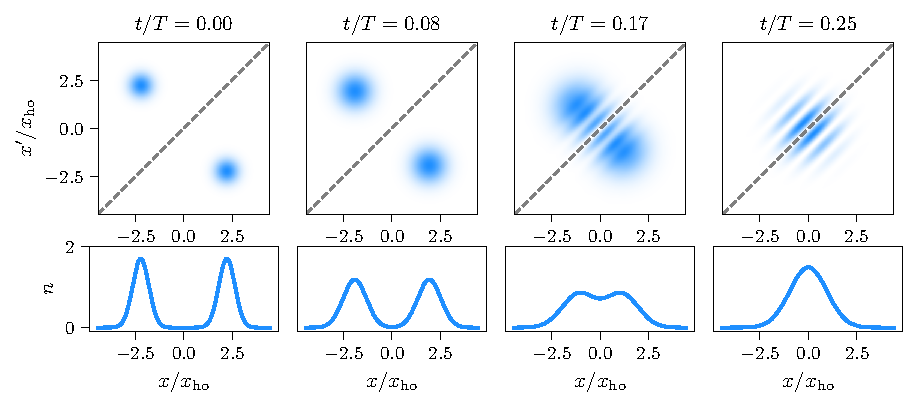
\includegraphics{fig-py/interference.pdf}
    \caption{
        \textbf{Two-fermion dynamics in a 1D harmonic trap: quantum statistics.}
        Top row: Time evolution of the two-particle correlation function $P_2(x,x')$ for two fermions in a harmonic potential. The characteristic anti-bunching dip along the diagonal reflects fermionic quantum statistics, contrasting the bunching peak expected for bosons. Bottom row: Corresponding single-particle density profiles $n(x)$, which remain indistinguishable from the bosonic case, highlighting the necessity of two-particle correlations to probe quantum statistics.
        }
    \label{fig:interference}
\end{figure}



\textbf{Split-step method.}
Complementing the classical Monte Carlo approach, in this work quantum mechanical simulations were employed to capture wavefunction dynamics during matter-wave magnification. Specifically, we utilize the split-step Fourier method, which efficiently solves the time-dependent Schrödinger equation, particularly suitable for systems with spatially varying potentials and wavefunction evolution.

The evolution of the atomic wavefunction $\psi(\vc{r}, t)$ is governed by the time-dependent Schrödinger equation:
\begin{equation*}
i\hbar\frac{\partial}{\partial t}\psi(\vc{r}, t) = \left(-\frac{\hbar^2}{2m}\nabla^2 + V(\vc{r})\right)\psi(\vc{r}, t).
\end{equation*}
The split-step method leverages the separation of kinetic and potential energy terms. The propagation over a timestep $\Delta t$ can be approximated by splitting the evolution operator into kinetic and potential contributions:
\begin{equation*}
\psi(\vc{r}, t + \Delta t) \approx e^{-i\frac{\Delta t}{2\hbar}V(\vc{r})} e^{-i\frac{\Delta t}{\hbar}\frac{\hat{p}^2}{2m}} e^{-i\frac{\Delta t}{2\hbar}V(\vc{r})}\psi(\vc{r}, t).
\end{equation*}

The kinetic operator is naturally handled in momentum space via the Fourier transform, as it becomes diagonal:
\begin{equation*}
\exp\left(-i\frac{\Delta t}{\hbar}\frac{\hat{p}^2}{2m}\right)\psi(\vc{r}, t) = \mathcal{F}^{-1}\left[\exp\left(-i\frac{\Delta t}{\hbar}\frac{\hbar^2 k^2}{2m}\right)\mathcal{F}{\psi(\vc{r}, t)}\right],
\end{equation*}
where $\mathcal{F}$ denotes the Fourier transform, and $k$ is the momentum-space coordinate. Thus, each evolution step avoids the stringent Courant–Friedrichs–Lewy (CFL) condition encountered in purely spatial methods, allowing for larger and more efficient timesteps.

Quantum treatment via the split-step method becomes particularly relevant when analyzing phenomena sensitive to quantum statistics. While average densities for ensembles of non-interacting atoms can be accurately captured using classical descriptions, quantum approaches are indispensable when studying relative positions of particles within individual realizations—especially for fermions. This is illustrated by considering two fermions in a harmonic trap, where quantum statistics significantly influence the spatial correlation patterns, producing characteristic anti-bunching behavior distinctly observable in the two-particle correlation function $P_2(x,x')$ \cite{bergschneider_experimental_2019}.

Specifically, the fermionic nature imposes Pauli exclusion, manifesting as a pronounced dip in $P_2(x,x')$ along the line $x=x'$, contrasting sharply with the bunching observed in bosonic systems. Such quantum-statistical features, shown explicitly in Fig.~\ref{fig:interference}, are not captured by classical simulations and underscore the necessity of quantum modeling methods like the split-step Fourier approach. Consequently, this technique complements the classical Monte Carlo simulations, providing a numerical framework to support the experimental realization of matter-wave magnification schemes described throughout this work.

The next subsection discusses in detail the Voronoi diagram-based method introduced to adaptively define regions of interest (ROI), mitigating spatial distortions inherent in the magnified atomic distributions.


\textbf{ROI with Voronoi diagrams.}
While matter-wave magnification significantly improves the spatial resolution for atomic imaging, practical implementations face challenges arising from anharmonicities and other distortions inherent in realistic trapping potentials. These distortions can lead to irregular spatial distributions, complicating reliable single-atom detection. Consequently, defining appropriate regions of interest (ROI) for each magnified atomic pattern becomes essential to ensure high detection fidelity.

In this work, a robust solution was introduced by employing Voronoi diagrams to adapt the ROI according to the actual spatial distributions observed after magnification. Voronoi diagrams partition a plane into distinct regions based on the distance to a specified set of points, known as "seeds". Each region contains exactly one seed, and any given point within a region is closer to its corresponding seed than to any other seed. Formally, for a set of seed points $\{\mathbf{s}_i\}$, the Voronoi region $R_i$ associated with seed $\mathbf{s}_i$ is defined as:
\begin{equation}
R\_i = {\mathbf{r} \mid |\mathbf{r}-\mathbf{s}\_i| \leq |\mathbf{r}-\mathbf{s}\_j|, \hspace{5 mm} \forall j \neq i}.
\end{equation}

By using the experimentally determined average final atom positions after the magnification process as seeds, Voronoi diagrams naturally provide adaptive ROIs tailored to distorted atom distributions. This ensures each ROI captures the atom signal associated with its corresponding trap site, even under anharmonic distortion. Voronoi-based ROI allocation minimizes signal contamination between neighboring sites, as each ROI is constructed explicitly to maximize separation from adjacent seed points, thereby reducing overlap.

Within the scope of this thesis, Voronoi diagram-based ROI adaptation was proposed and validated as a method for improving atom detection reliability after MWM. As demonstrated in Fig.~\ref{fig:mwm}b, applying Voronoi diagrams enhances detection by systematically accounting for magnification-induced distortions in atomic distributions. 


\textbf{Summary}. In this subsection, the concept of matter-wave magnification (MWM) was introduced, a powerful approach to enhance spatial resolution in quantum gas microscopy beyond conventional optical limitations.
To accurately describe and optimize the MWM process, two numerical methodologies were implemented. The classical Monte Carlo approach with fourth-order Runge-Kutta (RK4) integration provides efficient simulation of large ensembles of atoms, effectively capturing macroscopic ensemble dynamics. In parallel, the split-step Fourier method addresses quantum-mechanical wavefunction evolution, essential when quantum-statistical effects such as fermionic anti-bunching become relevant. Distortions induced by potential anharmonicities were addressed using Voronoi diagrams. This adaptive method adjusts regions of interest based on observed atomic distributions, ensuring robust atom detection even under realistic experimental conditions.

% Collectively, these numerical tools and conceptual advances substantially enhance the feasibility and accuracy of matter-wave magnification experiments. Future work will focus on refining potential designs and further exploring quantum-statistical phenomena, particularly in fermionic systems. These developments open promising avenues for deeper investigations into quantum correlations, transport dynamics, and non-equilibrium physics in ultracold atomic systems.
 % Monte Carlo simulation, wavefunction evolution

\subsection{Determinantal Point Processes}
% !TEX root = ../master-thesis.tex




% Pauli crystall \cite{holten_observation_2021}

% DPP: \cite{kulesza_determinantal_2012}, \cite{hough_determinantal_2006}

A central challenge in quantum many-body systems involving indistinguishable fermionic particles is the accurate modeling of the fermionic antisymmetry in the many-body wavefunction. Even in the case of non-interacting fermions, the generation of realistic samples of experimentally observable quantities—such as single-shot atomic density measurements—requires proper antisymmetrization. As the number of particles and the dimensionality of the system increase, enforcing these antisymmetric constraints becomes computationally demanding. For example, treating antisymmetric wavefunctions explicitly for as few as four fermions in two dimensions already presents nontrivial computational difficulties.

To mitigate this challenge, Determinantal Point Processes (DPPs) are employed as a probabilistic framework inherently suited to capturing fermionic statistics. DPPs naturally model repulsive correlations between particles, reflecting the Pauli exclusion principle, and provide a mathematically principled and computationally efficient approach for sampling particle configurations from single-particle wavefunctions.

In experiments reporting the observation of "Pauli crystals"—ordered spatial structures emerging solely from quantum statistical effects—analytical sampling expressions have been derived under restrictive symmetry assumptions. However, in broader experimental contexts, such analytical forms are typically unavailable. In these cases, the DPP-based approach offers a general-purpose numerical method for simulating atomic distributions across diverse trapping geometries.

The following sections present a formal mathematical description of Determinantal Point Processes, detail the algorithmic procedures for DPP sampling, and compare the computational efficiency with that of direct antisymmetrization. The method’s practical utility is illustrated through numerical examples, including the reproduction of characteristic correlation features (see Fig.\ref{fig:interference}) using DPP-based simulations (see Fig.\ref{fig:interference-dpp}).

\begin{figure}
    \centering
    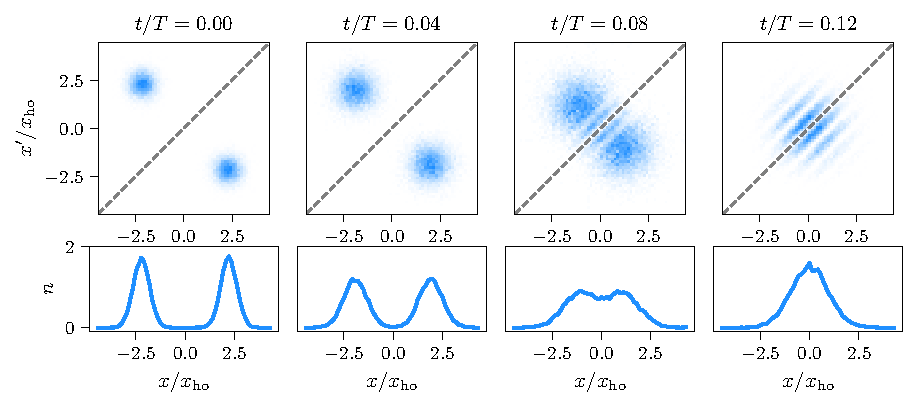
\includegraphics{fig-py/interference_dpp.pdf}
    \caption{DPP based}
    \label{fig:interference-dpp}
\end{figure}


\textbf{Mathematical formulation.}
Formally, a Determinantal Point Process on a space $\Lambda$ equipped with a suitable reference measure $\mu$ is defined through a kernel function $K(x,y)$, where $x,y \in \Lambda$. For a DPP, the probability of observing a configuration of points $\{x_1, x_2, \ldots, x_n\}$ is proportional to the determinant of a corresponding kernel matrix formed by evaluating $K$ at these points:
\begin{equation}
P(x_1, x_2, \ldots, x_n) \propto \det[K(x_i, x_j)]_{1 \leq i,j \leq n}.
\end{equation}
This determinantal structure naturally encodes repulsive correlations between points, making DPPs particularly well-suited for modeling fermionic systems where identical particles exhibit antisymmetric quantum statistics. Specifically, the kernel $K(x,y)$ typically corresponds to the two-point correlation function derived from the underlying single-particle wavefunctions:
\begin{equation}
K(x, y) = \sum_{k} \lambda_k \phi_k(x)\phi_k^*(y),
\end{equation}
where $\{\phi_k\}$ form an orthonormal set of eigenfunctions of a corresponding integral operator, and $\{\lambda_k\}$ are the associated eigenvalues, bounded between 0 and 1 to guarantee the existence of the process \cite{hough_determinantal_2006}.

The fundamental advantage of DPPs lies in their efficient sampling procedure, which bypasses the combinatorial complexity of directly antisymmetrizing wavefunctions. Specifically, if the kernel represents a projection operator (i.e., $\lambda_k$ equals either 0 or 1), the DPP simplifies to a projection DPP, significantly enhancing computational tractability.

% Sampling algorithm section

Given a projection kernel $K$, the sampling procedure of a projection DPP begins by computing the eigen-decomposition of the kernel $K$:
\begin{equation}
K(x,y) = \sum_{k=1}^{M} \phi_k(x)\phi_k^*(y),
\end{equation}
where $\{\phi_k\}$ form an orthonormal basis of the subspace associated with eigenvalue 1.
The algorithm then initializes an empty set $Y$ and proceeds iteratively. At each iteration, selection probabilities are computed proportional to:
\begin{equation}
p(x) = \frac{1}{M} \sum_{k=1}^{M} |\phi_k(x)|^2.
\end{equation}
A point $x$ is selected according to $p(x)$, after which the subspace is updated by projecting out the selected function:
\begin{equation}
\phi_k(x) \rightarrow \phi_k(x) - \sum_j \frac{\phi_j(x_{\text{selected}})}{\phi_j(x)} \phi_k(x_{\text{selected}}),
\end{equation}
and the resulting basis set is renormalized. The selected point is added to $Y$, $M$ is decreased, and the process repeats until $M = 0$. This approach efficiently generates sample realizations that adhere to the correct fermionic antisymmetry without explicitly antisymmetrizing wavefunctions.

% Computational complexity section
% \section*{\textbf{Computational complexity}}

Direct antisymmetrization of wavefunctions involves computing determinants of large matrices for every possible configuration, resulting in computational complexity that scales factorially with the particle number. In contrast, the projection-DPP sampling method described above significantly reduces complexity. It scales polynomially in both the number of points sampled and the number of eigenfunctions, typically providing practical feasibility for experimental scenarios involving tens or hundreds of particles.

Nevertheless, obtaining the eigen-decomposition of the kernel can become computationally intensive for large continuous spaces. Therefore, numerical implementations typically utilize efficient algorithms and GPU acceleration to handle realistic experimental scales, as demonstrated earlier in this thesis. The application of this DPP sampling approach was illustrated by replicating the quantum correlation results previously shown in Fig.~\ref{fig:interference}, demonstrating how realistic experimental snapshots can be efficiently generated using Determinantal Point Processes (Fig.~\ref{fig:interference-dpp}).
 


% \newpage

\subsection{\red{Some data}}
% !TEX root = ../master-thesis.tex

\textbf{From frequency to position}. И в camera based balancing, и в atoms based balancing для обработки изображений удобно определить афинное преобразование из frequency space to position space:
\begin{equation*}
	\vc{r} = H \vc{\omega}
	\hspace{5 mm} \leftrightarrow \hspace{5 mm} 
	\begin{pmatrix}
		x \\ y
	\end{pmatrix} = \begin{pmatrix}
		h_{11} & h_{12} & h_{13} \\
		h_{21} & h_{22} & h_{23} \\
	\end{pmatrix} 
	\begin{pmatrix}
		\sub{\omega}{hor} \\
		\sub{\omega}{ver} \\
		1
	\end{pmatrix}.
\end{equation*}
Можно, например, для случайных $\vc{\omega}_j \in [\sub{\omega}{min},\, \sub{\omega}{max}]$ измерить $\vc{r}_j$, таким образом сформировав две матрицы $\omega_{ij}$ with $i \in \{\mathrm{hor},\, \mathrm{ver}\}$ and $r_{ij}$ with $i \in \{x, y\}$. Остается решить уравнение на $H$ (что соответсвует Least squares method):
\begin{equation}
	r = H \omega,
	\hspace{0.5cm} \Rightarrow \hspace{0.5cm}
	r \omega\T = H \omega \omega\T
	\hspace{0.5cm} \Rightarrow \hspace{0.5cm}
	r \omega\T \left(\omega \omega\T\right)^{-1} = H.
	\label{LinReg:freq2pos}
\end{equation}


\newpage
\bibliographystyle{plain}
\bibliography{master-thesis.bib}


\end{document}


